\chapter{量子跃迁}\label{chp:09}
% \makebox[5em][s]{} % 短题目拉间距

% 与时间有关的微扰论
\section[与时间有关的微扰论]{与时间有关的微扰论} \label{sec:09.01} % 
% \makebox[5em][s]{} % 短题目拉间距

考虑一个物理体系(例如一个原子),其能量算符为$H_{0}$(不显含$t$),$H_{0}$的正交归一化的本征函数记为$\varPsi_{n}(x)$,相应的能级记为$E_{n}$.[$x$代表波函数所涉及的全体独立变量,也可以理解为某种守恒量完全集($H_{0}$在内)的共同本征函数,$n$代表全体量子数.]设开始时体系处于定态$\varPsi_{k}$.如果没有外界作用,体系将继续处于$\varPsi_{k}$态,波函数的时间变化表现为一个位相因子,
\begin{empheq}{equation}\label{eq91.1}
	\varPsi_{k}(x,t)=\varPsi_{k}(x)e^{-iE_{k}t/\hbar}
\end{empheq}
这就是定态.

设$t>0$时体系受到外界作用,作用势$H^{\prime}(x,t)$,即体系的总能量算符变成
\eqshort
\begin{empheq}{equation}\label{eq91.2}
	H=H_{0}+H^{\prime}
\end{empheq}\eqnormal
设$[H_{0},H^{\prime}]\neq0$,因此$t>0$时$H_{0}$不再是守恒量.与此相应,波函数满足薛定谔方程:
\begin{empheq}{equation}\label{eq91.3}
	i\hbar\frac{\partial}{\partial t}\varPsi(x,t)=H\varPsi=(H_{0}+H^{\prime})\varPsi(x,t)
\end{empheq}
按照态叠加原理,$\varPsi(x,t)$可以表示成$H_{0}$的本征函数的线性叠加,即
\begin{empheq}{equation}\label{eq91.4}
	\varPsi(x,t)=\sum_{n}C_{n}(t)\varPsi_{n}(x)e^{-iE_{n}t/\hbar}
\end{empheq}
初始条件为
\begin{empheq}{equation}\label{eq91.5}
	\varPsi(x,0)=\varPsi_{k}(x)\quad\text{即}\quad C_{n}(0)=\delta_{nk}
\end{empheq}
如求出了各$C_{n}(t)$,也就是求出了$\varPsi(x,t)$.设在$t=T$时去除外界作用$H^{\prime}$,并随即测量体系的能量,即测量$H_{0}$,按照波函数的普遍概率解释,测得$H_{0}=E_{f}$的概率为$C_{f}^{*}(T)C_{f}(T)$,这也就是$t=T$时体系处于$\varPsi_{f}$态的概率.或者说,$C_{f}^{*}(T)C_{f}(T)$就是到时刻$T$为止体系已由原先的$\varPsi_{k}$态跃迁到$\varPsi_{f}$态的概率.$C_{f}^{*}C_{f}$的时间变化率称为由$\varPsi_{k}$态变到$\varPsi_{f}$态的跃迁速率,记为
\begin{empheq}{equation}\label{eq91.6}
	w_{k\rightarrow f}(t)=\frac{d}{dt}[C_{f}^{*}(t)C_{f}(t)]
\end{empheq}
$\varPsi_{k}$称为初态,$\varPsi_{f}$称为终态.

为了求出$C_{f}(t)$,将\eqref{eq91.4}式代入\eqref{eq91.3}式,得到
\begin{empheq}{equation*}
	i\hbar\sum_{n}\frac{dC_{n}}{dt}\varPsi_{n}e^{-iE_{n}t/\hbar}=\sum_{n}H^{\prime}\varPsi_{n}C_{n}e^{-iE_{n}t/\hbar}
\end{empheq}
以$\varPsi_{f}^{\prime}$左乘上式,对全空间积分,并注意利用正交归一化条件
\begin{empheq}{equation}\label{eq91.7}
	\int\varPsi_{f}^{*}(x)\varPsi_{n}(x)dx=\delta_{fn}
\end{empheq}
可得
\begin{empheq}{equation}\label{eq91.8}
	i\hbar\frac{dC_{f}}{dt}e^{-E_{f}t/\hbar}=\sum_{n}H_{fn}^{\prime}C_{n}e^{-iE_{n}t/\hbar}
\end{empheq}
其中
\begin{empheq}{equation}\label{eq91.9}
	H_{fn}^{\prime}=\int\varPsi_{f}^{*}H^{\prime}\varPsi_{n}dx=\langle \varPsi_{f}|H^{\prime}|\varPsi_{n} \rangle 
\end{empheq}
是$H_{0}$表象中$H^{\prime}$的矩阵元,它与时间$t$有关.

\eqref{eq91.8}式是严格的,它代表一组联立方程$(f=1,2,\cdots)$,如能严格解出,当然很好.但一般\eqref{eq91.8}式不易严格解出,需用近似解法.本节只介绍微扰论解法,条件是$H^{\prime}$较弱而且作用时间也不长,时刻$t$时体系已由初态$\varPsi_{k}$跃迁到各个可能终态的总概率远小于1,即
\begin{empheq}{equation}\label{eq91.10}
	\sum_{n}^{\prime}C_{n}^{*}(t)C_{n}(t)\ll 1
\end{empheq}
在这条件下可以略去\eqref{eq91.8}式右端所有$n\neq k$的$C_{n}$,并取$C_{k}(t)\approx1$,从而将\eqref{eq91.8}式近似为
\begin{empheq}{equation}\label{eq91.11}
	i\hbar\frac{d}{dt}C_{f}=H_{fk}^{\prime}(t)e^{i\omega_{fk}t}
\end{empheq}
积分,即得满足初始条件\eqref{eq91.5}式的解为
\begin{empheq}{equation}\label{eq91.12}
	\boxed{C_{f}(t)=\frac{1}{i\hbar}\int_{0}^{t}H_{fk}^{\prime}e^{i\omega_{fk}t}dt}
\end{empheq}
其中$\omega_{fk}=\frac{E_{f}-E_{k}}{\hbar}$.这个结果相当于视$H^{\prime}$为微扰而求出的一级近似.如将\eqref{eq91.12}式再代入\eqref{eq91.8}式右端(令$f\rightarrow n$),就可求出$C_{f}(t)$的二级近似.不过通常只取一级近似,即\eqref{eq91.12}式,这是本章的基本公式.

从\eqref{eq91.12}式可知,如果$H_{fk}^{\prime}(t)=0(0<t<T)$则$C_{f}(t)=0$,即由$\varPsi_{k}$态到$\varPsi_{f}$态的跃迁是禁戒的.为了使跃迁$\varPsi_{k}\rightarrow\varPsi_{f}$成为可能,须$H_{fk}^{\prime}\neq0$,为此而出现的量子数$f$与$n$间的制约关系即所谓选择定则.

如果考虑反方向的跃迁过程,即初态为$\varPsi_{f}$,终态为$\varPsi_{k}$,重复上述计算,$C_{k}$的公式显然只需在\eqref{eq91.12}式中将$f$、$k$互换.由于$H^{\prime}$应该是厄密的$(H^{\prime}=H^{\prime+})$,必有$H_{kf}^{\prime}=(H_{fk}^{\prime})^{*}$,因此现在问题中的$-C_{k}(t)$等于\eqref{eq91.12}式决定的$C_{f}^{*}(t)$.这就是说,在同一种外界作用下($H^{\prime}$相同),$\varPsi_{k}\rightarrow\varPsi_{f}$及$\varPsi_{f}\rightarrow\varPsi_{k}$这两种正、反跃迁过程的跃迁速率相等.
\pskip

\example 有一个量子力学体系,总能量算符$H_{0}$的本征函数(已正交归一化)为$\varPsi_{n}(x)$,能级$E_{n},n=1,2,\cdots$.已知$t<0$时体系处于基态$\varPsi_{k}$,$t>0$时受到外来微扰$H^{\prime}(x,t)=F(x)e^{-t/\tau}$的作用.试用微扰论(一级近似)求$t\gg\tau$时$(t\rightarrow\infty)$体系处于各激发态$(\varPsi_{n},E_{n}>E_{1})$的概率.

\solution 微扰$H^{\prime}$的矩阵元($H_{0}$表象)为
\begin{empheq}{align*}
	H_{n1}^{\prime}(t) &=e^{-t/\tau}\int\varPsi_{n}^{*}(x)F(x)\varPsi_{1}(x)dx	\\
	&=F_{n1}e^{-t/\tau}
\end{empheq}
如$F_{n1}\neq0$,$H^{\prime}$将引起由$\varPsi_{k}$向$\varPsi_{n}$的跃迁,所求概率等于$C_{n}^{*}(\infty)C_{n}(\infty)$.按照\eqref{eq91.12}式,
\begin{empheq}{align*}
	C_{n}(t) &=\frac{F_{n1}}{i\hbar}\int_{0}^{t}\exp\left(i\omega_{n1}t-\frac{t}{\tau}\right)dt	\\
	&=\frac{\frac{F_{n1}}{i\hbar}\left[\exp\left(i\omega_{n1}t-\frac{t}{\tau}\right)-1\right]}{i\omega_{n1}-\frac{1}{\tau}}
\end{empheq}
当$t\rightarrow\infty(t\gg\tau)$,即得
\begin{empheq}{equation*}
	C_{n}(\infty)=\frac{F_{n1}}{E_{n}-E_{1}+\frac{i\hbar}{\tau}}
\end{empheq}
体系处于$\varPsi_{n}$态的概率为
\begin{empheq}{equation*}
	|C_{n}(\infty)|^{2}=\frac{|F_{n1}|^{2}}{(E_{n}-E_{1})^{2}+\frac{\hbar^{2}}{\tau^{2}}}
\end{empheq}
微扰论适用条件为$\sum^{\prime}|C_{n}|^{2}\gg1(n\neq1)$,为此必须$|C_{n}|^{2}\gg1$,即
\begin{empheq}{equation*}
	|F_{n1}|\gg E_{n}-E_{1}\quad\text{或}\quad |F_{n1}|\gg\frac{\hbar}{\tau}
\end{empheq}









% 几种典型跃迁
\section[几种典型跃迁]{几种典型跃迁} \label{sec:09.02} % 
% \makebox[5em][s]{} % 短题目拉间距

{\heiti 1.初、终态属于分立能谱,$H^{\prime}$为单频微扰}

设$t>0$时微扰$H^{\prime}$是单频的:
\begin{empheq}{align}\label{eq92.1}
	H^{\prime} &=\hat{F}(x)2\cos\omega_{0}t	\nonumber\\
	&=\hat{F}(x)(e^{i\omega_{0}t}+e^{-i\omega_{0}t})
\end{empheq}
其中$\hat{F}$为与时间无关的厄密算符.$(\hat{F}=\hat{F}^{+})$跃迁过程则完全按照$\S$\ref{sec:09.01}的提法,为了便于讨论,设终态能级片高于初态能级,即

微扰$H^{\prime}$的矩阵元为
\begin{empheq}{align}\label{eq92.2}
	H_{fk}^{\prime} &=\langle \varPsi_{f}|H^{\prime}|\varPsi_{k}\rangle \nonumber\\
	&=F_{fk}(e^{i\omega_{0}t}+e^{-i\omega_{0}t})
\end{empheq}
其中
\begin{empheq}{equation}\label{eq92.3}
	F_{fk}=\langle \varPsi_{f}|\hat{F}|\varPsi_{k}\rangle=\int\varPsi_{f}^{*}\hat{F}(x)\varPsi_{k}(x)dx
\end{empheq}
按照\eqref{eq91.12}式,容易求出
\eqindent{1}
\begin{empheq}{align}\label{eq92.4}
	C_{f}(t) &=\frac{F_{fk}}{i\hbar}\int_{0}^{t}(e^{i\omega_{0}t}+e^{-i\omega_{0}t})e^{i\omega_{fk}t}dt	\nonumber\\
	&=\frac{F_{fk}}{i\hbar}\left\{\frac{\exp[it(\omega_{fk}+\omega_{0})]-1}{i(\omega_{fk}+\omega_{0})}+\frac{\exp[it(\omega_{fk}-\omega_{0})]-1}{i(\omega_{fk}-\omega_{0})}\right\}
\end{empheq}\eqnormal
通常对跃迁概率进行测量的时刻,$H^{\prime}$已经作用了许多个周期,即总是满足条件$\omega_{0}t\gg2\pi$(以光波作用于原子为例,$\omega_{0}$约为$10^{15}\sim10^{16}\si{s^{-1}}$,当$t>10^{-13}\si{s}$,就满足这条件.)\eqref{eq92.4}式中分母为$(\omega_{fk}+\omega_{0})$的项可以略去,即取
\begin{empheq}{equation*}\label{eq92.4'}
	C_{f}(t)\approx\frac{F_{fk}}{\hbar}\cdot\frac{1-\exp[it(\omega_{fk}-\omega_{0})]}{\omega_{fk}-\omega_{0}}	\tag{$9.2.4^{\prime}$}
\end{empheq}
于是可得
\eqllong
\begin{empheq}{equation}\label{eq92.5}
	C_{f}^{*}(t)C_{f}(t)\approx\frac{|F_{fk}|^{2}}{\hbar^{2}}\frac{2}{(\omega_{fk}-\omega_{0})^{2}}[1-\cos(\omega_{fk}-\omega_{0})t]
\end{empheq}\eqnormal
跃迁速率为
\begin{empheq}{align}\label{eq92.6}
	w_{k\rightarrow f} &=\frac{d}{dt}[C_{f}^{*}(t)C_{f}(t)]	\nonumber\\
	&=\frac{2}{\hbar}|F_{fk}|^{2}\frac{\sin(\omega_{fk}-\omega_{0})t}{\omega_{fk}-\omega_{0}}
\end{empheq}
显然,仅当$\omega_{fk}\sim\omega_{0}$时,\eqref{eq92.6}式才有显著的值.利用公式
\begin{empheq}{equation}\label{eq92.7}
	\delta(x)=\frac{1}{2\pi}\int_{-\infty}^{\infty}e^{ikx}dk=\frac{\sin\alpha x}{\pi x}\quad (\alpha\rightarrow\infty)
\end{empheq}
可以对\eqref{eq92.6}式取下列近似
\begin{empheq}{equation}\label{eq92.8}
	\frac{\sin(\omega_{fk}-\omega_{0})t}{\pi(\omega_{fk}-\omega_{0})}\approx\delta(\omega_{fk}-\omega_{0})
\end{empheq}\eqlong
\begin{empheq}{align}\label{eq92.9}
	w_{k\rightarrow f}(t)\approx& \frac{2\pi}{\hbar^{2}}|F_{fk}|^{2}\delta(\omega_{fk}-\omega_{0})	\nonumber\\
	&=\frac{2\pi}{\hbar}|F_{fk}|^{2}\delta(E_{f}-E_{k}-\hbar\omega_{0})
\end{empheq}\eqnormal
其中$\delta$函数表明,仅当$(E_{f}-E_{k})=\hbar\omega_{0}$,跃迁速率才可能不为0,这正是能量守恒定律在跃迁过程中的具体体现.注意,跃迁速率$w_{k\rightarrow f}$与$t$无关(但必须以\eqref{eq92.8}式成立为前提),这时$C_{f}^{*}C_{f}$与$t$成正比,即
\eqshort
\begin{empheq}{equation}\label{eq92.10}
	C_{f}^{*}(t)C_{f}(t)\approx tw_{k\rightarrow f}
\end{empheq}\eqnormal
这表明$\varPsi_{k}\rightarrow\varPsi_{f}$跃迁过程在宏观时间尺度上是匀速进行的.

{\heiti 2.终态能级$E_{f}$属于连续能谱,$H^{\prime}$为单频微扰}

\begin{wrapfigure}[12]{r}{7em}
	\centering
	\small
	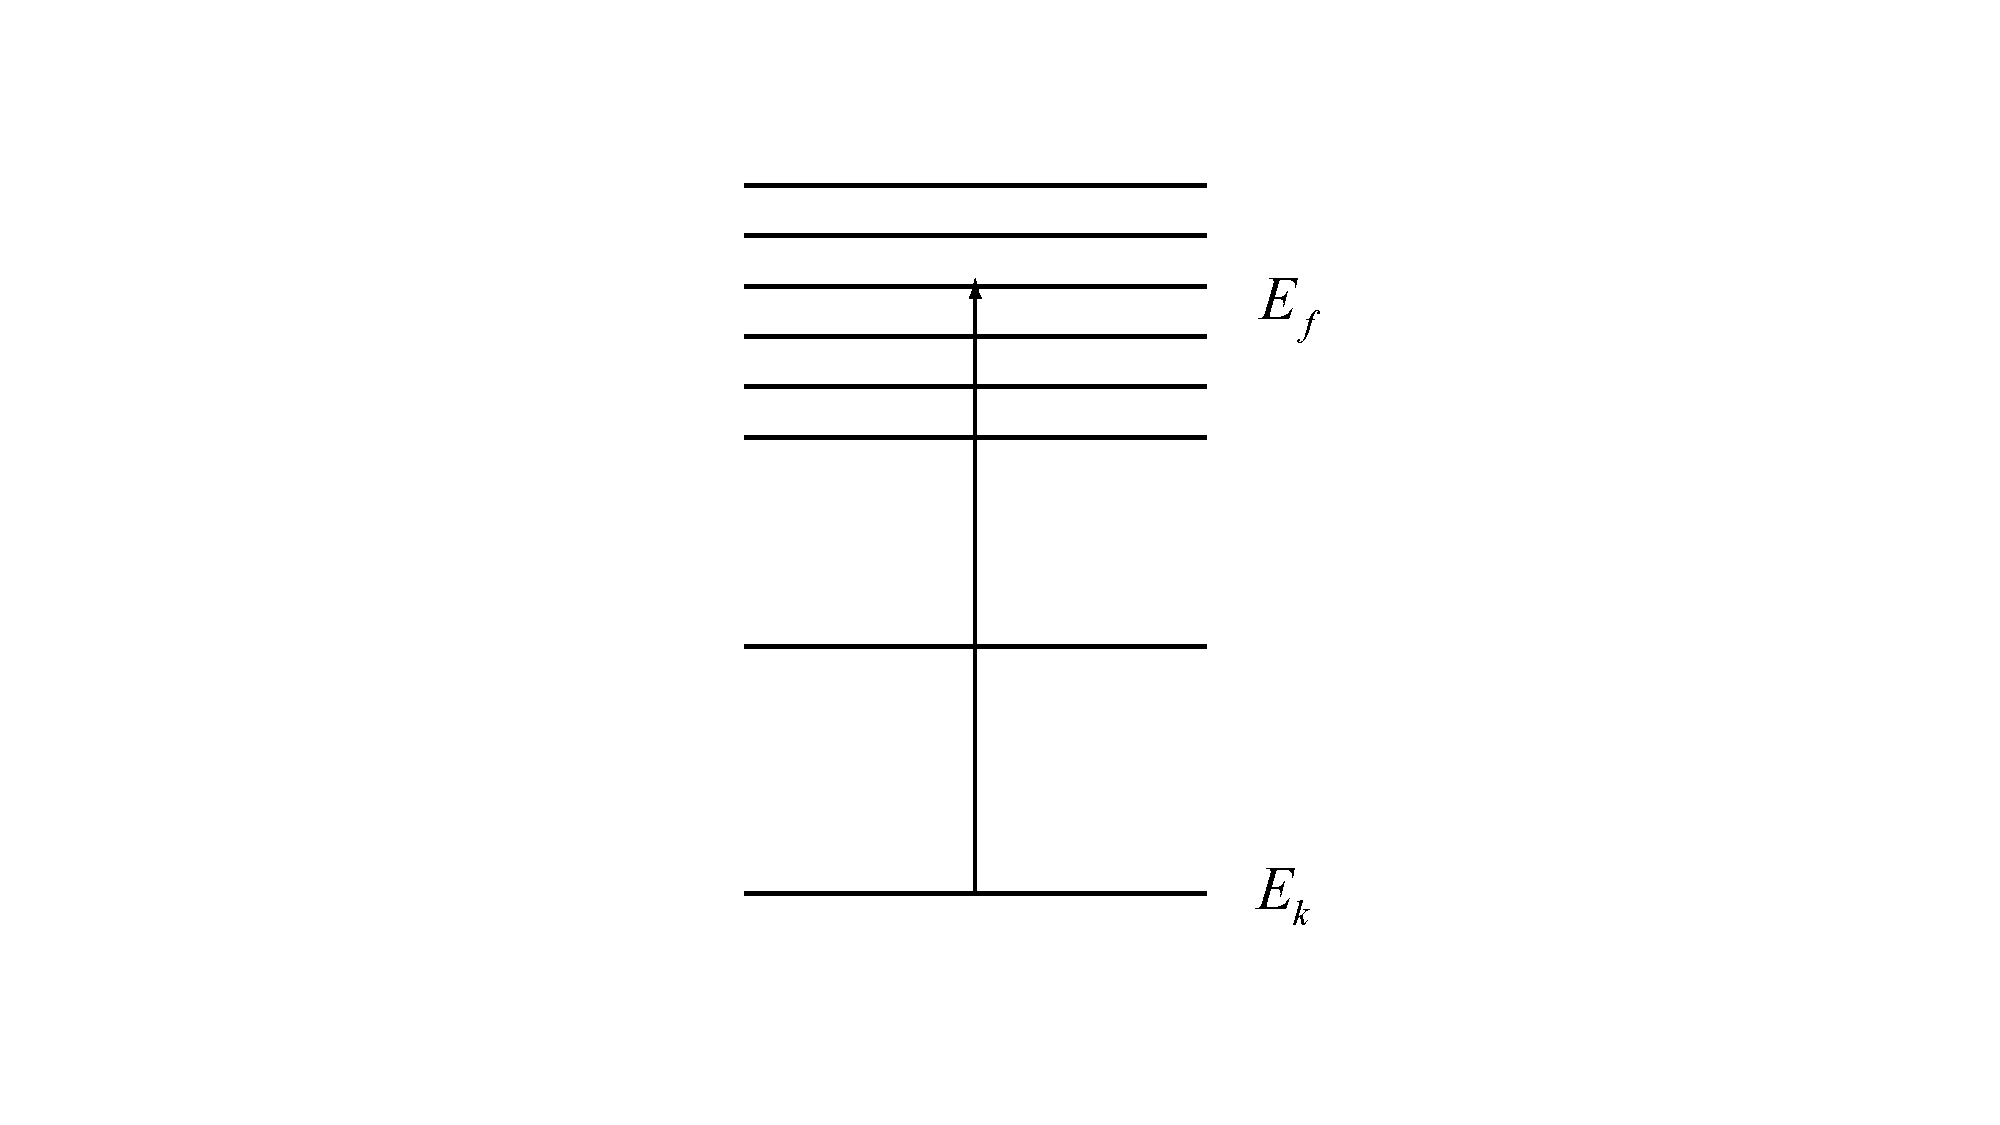
\includegraphics[width=3cm,clip]{QM file/figure/9-1}
	\caption{}\label{fig.9-1}
\end{wrapfigure}

仍设$H^{\prime}$为单频并取\eqref{eq92.1}式之形式.

连续能谱可以认为是能级密集的极限情形,如图\ref{fig.9-1}所示.由于终态能级密集,严格区分终态能量的微小差别既无可能,也无必要.有实际意义的做法是计算从初态$\varPsi_{k}$跃迁到能量接近$(E_{k}+\hbar\omega_{0})$的各个终态的概率总和.设在$E_{f}\approx(E_{k}+\hbar\omega_{0})$附近,能量范围$dE_{f}$内状态数为$\rho(E_{f})dE_{f}$,$\rho(E_{f})$称为状态密度.则由初态$\varPsi_{k}$向这些终态的跃迁速率总和为
\eqlong
\begin{equation}\label{eq92.11}
	W_{k\rightarrow f}=\int w_{k\rightarrow f}\rho(E_{f})dE_{f}
\end{equation}
将\eqref{eq92.9}式代入上式,得到
\begin{empheq}{equation}\label{eq92.12}
	\boxed{	W_{k\rightarrow f}=\frac{2\pi}{\hbar}|F_{fk}|^{2}\rho(E_{f}),\quad E_{f}=E_{k}+\hbar\omega_{0}	}
\end{empheq}\eqnormal
这公式有时称为黄金规则.在以上推导中假定$dE_{f}$范围内各个终态除能量略有差别外,其他方面的性质相同,特别是$F_{fk}$相同,这样由\eqref{eq92.11}式就得到\eqref{eq92.12}式.如果这些终态的$F_{fk}$有几种取值,则应按$F_{fk}$的数值将终态分类,对各类终态分别计算其状态密度和跃迁速率.

用紫外线(角频率$\omega_{0}$)照射原子,使原子中电子$(E_{k}<0)$电离$(E_{f}>0)$的过程(光电效应)就是属于本节讨论的问题.

{\heiti 3.常微扰}

设$t>0$时$H^{\prime}=H^{\prime}(x)$,与$t$无关这种情况相当于$\omega_{0}\rightarrow0$,只需在以上各公式中将$F_{fk}$换成$H_{fk}^{\prime}$,并取$\omega_{0}=0$就行了.例如\eqref{eq92.9}式改为
\begin{empheq}{equation}\label{eq92.13}
	w_{k\rightarrow f}\approx\frac{2\pi}{\hbar}|H_{fk}^{\prime}|^{2}\delta(E_{f}-E_{k})
\end{empheq}
其中$\delta$函数表明跃迁只能在能量相同的状态间发生.对于分立能级,常微扰将引起各简并态相互跃迁,结果导致这些简并态重新组合,形成新的定态.但如有某个简并态$\varPsi_{k}$,它与其他所有简并态(各$\varPsi_{f}$)之间$H_{fk}^{\prime}$均等于0,则$\varPsi_{k}$将不受微扰$H^{\prime}$的影响而保待其独立性,即在$H=H_{0}+H^{\prime}$的情况下,$\varPsi_{k}$仍是正确的定态波函数(在零级近似程度上,参看$\S$\ref{sec:06.02}).

\pskip
\example 弹性散射

按照量子跃迁的观点处理弹性散射,可以很便捷地导出散射截面的玻恩近似公式,如下.

\begin{figure}[!h]
	\centering
	\small
	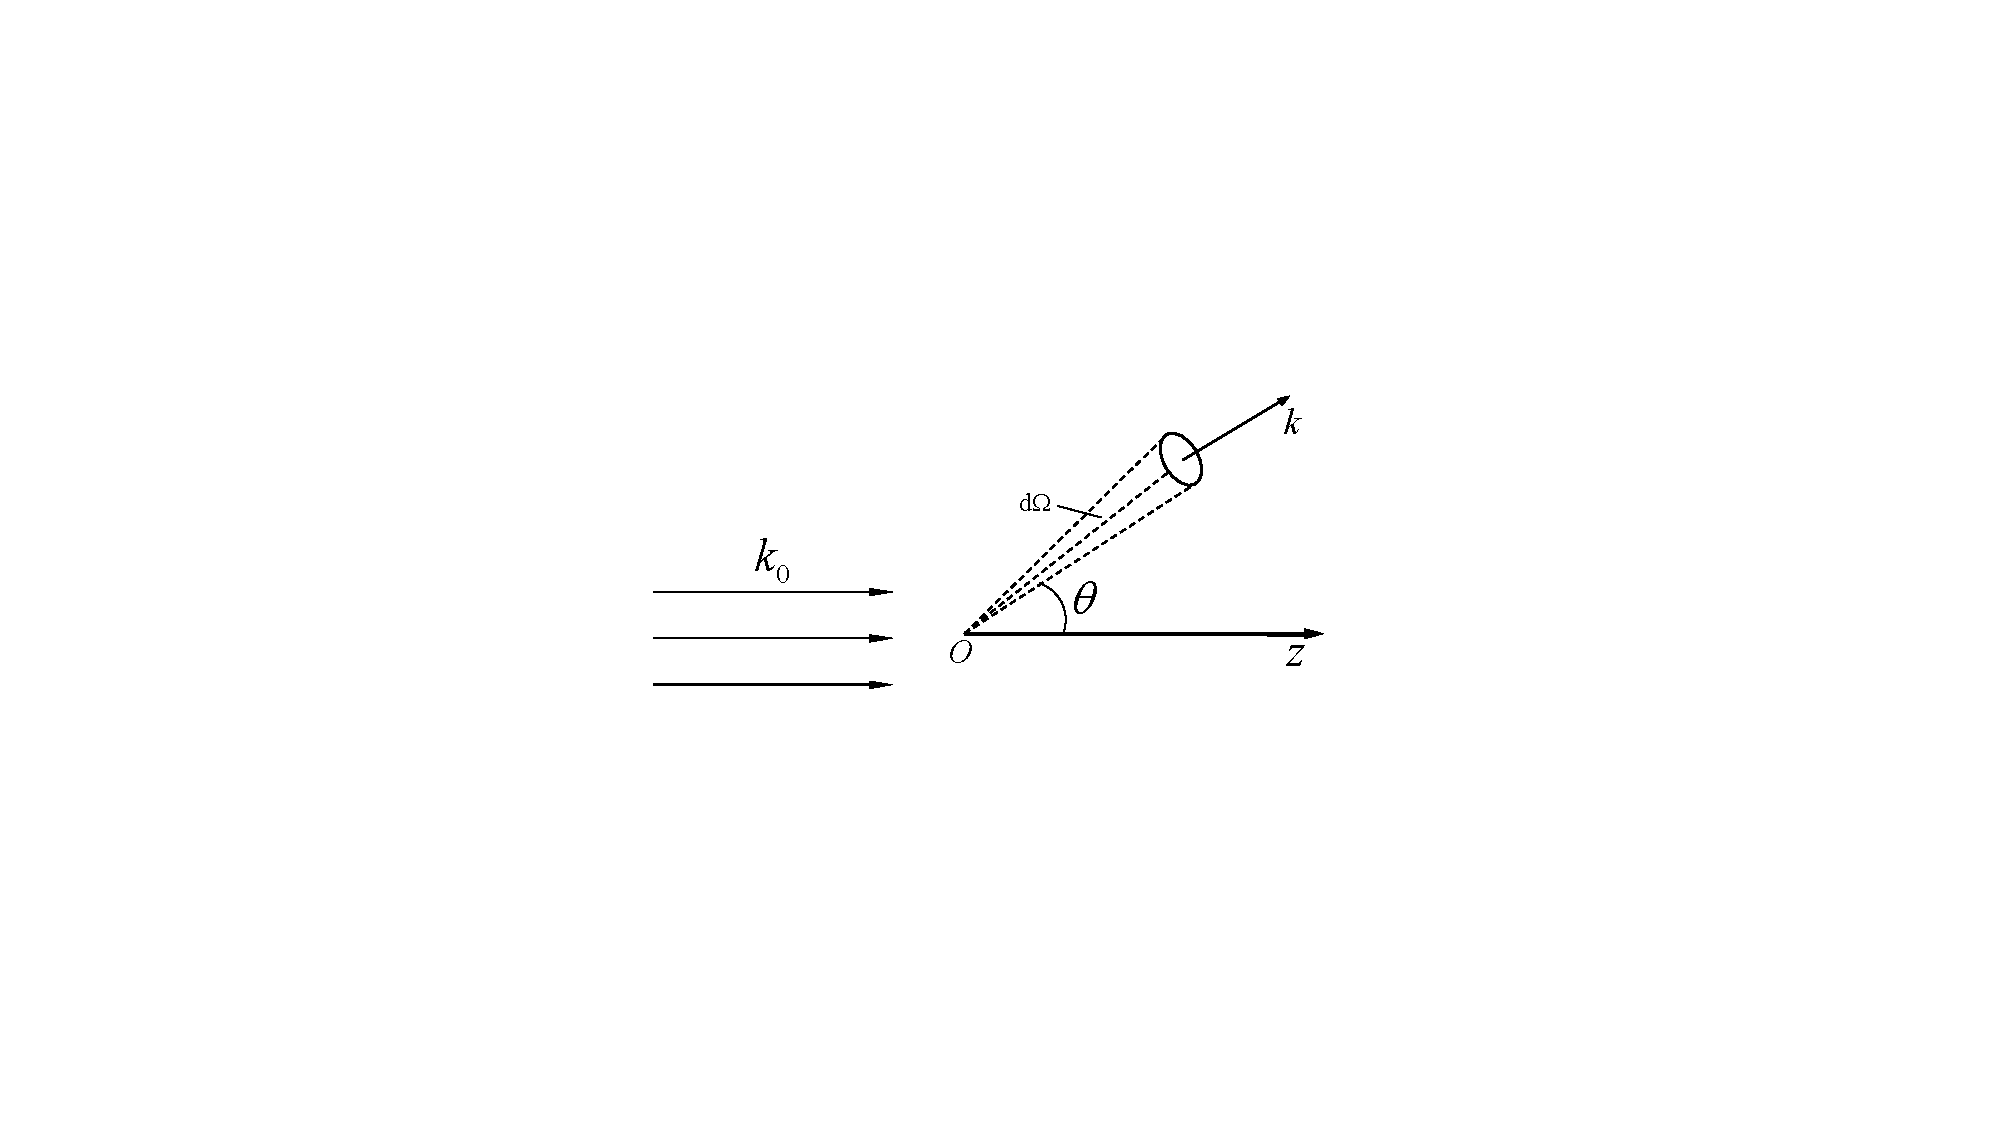
\includegraphics[width=6cm,clip]{QM file/figure/9-2}
	\caption{}\label{fig.9-2}
\end{figure}

散射过程中粒子的动量变化如图\ref{fig.9-2}所示.入射动量$\hbar k_{0}$,出射动量$\hbar k$,散射角$\theta$.为了便于计算状态密度,采用“箱归一化”方法($\S$\ref{sec:03.05}),“箱子”体积$L^{3}$.归一化的初态和终态波函数为
\begin{empheq}{align}
	\varPsi_{k_{0}}(\boldsymbol{r})=&L^{-\frac{3}{2}}e^{ik_{0}z}=L^{-\frac{3}{2}}e^{i\boldsymbol{k}_{0}\cdot\boldsymbol{r}}	\label{eq92.14}\\
	&\varPsi_{k}(\boldsymbol{r})=L^{-\frac{3}{2}}e^{i\boldsymbol{k}\cdot\boldsymbol{r}}	\label{eq92.15}
\end{empheq}
散射作用势视为常微扰,即令
\eqshort
\begin{empheq}{equation}\label{eq92.16}
	H^{\prime}=V(\boldsymbol{r})
\end{empheq}\eqnormal
在$V(\boldsymbol{r})$作用下粒子被散射到$(\theta,\varphi)$方向,相当于从初态$\varPsi_{k_{0}}$跃迁到终态$\varPsi_{k}$,由于终态动量$\hbar k$可以连续变化,应按连续谱处理,终态动量方向在$(\theta,\varphi)$附近$d\Omega$范围内的状态数为[参看\eqref{eq35.34}式]
\begin{empheq}{equation}\label{eq92.17}
	\rho(E)dE=\frac{L^{3}d^{3}\boldsymbol{p}}{h^{3}}=\frac{L^{3}\boldsymbol{p}^{2}dpd\Omega}{h^{3}}
\end{empheq}
终态动量与能量间有关系
\begin{empheq}{equation}\label{eq92.18}
	E=\frac{p^{2}}{2\mu},\quad dE=\frac{pdp}{\mu}
\end{empheq}
代入\eqref{eq92.17}式,即得
\begin{empheq}{equation}\label{eq92.19}
	\rho(E)=\frac{L^{3}\mu pd\Omega}{h^{3}}
\end{empheq}

由初态$\varPsi_{k_{0}}$跃迁到终态动量方向在$d\Omega$范围内的一切终态,跃迁速率总和可以按\eqref{eq92.12}式计算,即
\eqlong
\begin{empheq}{equation}\label{eq92.20}
	W=\frac{2\pi}{\hbar}|V_{kk_{0}}|^{2}\rho(E)=\frac{2\pi}{\hbar h^{3}}L^{3}\mu pd\omega|V_{kk_{0}}|^{2}
\end{empheq}\eqnormal
其中
\begin{empheq}{align}\label{eq92.21}
	V_{kk_{0}} &=\langle \varPsi_{k}|V|\varPsi_{k_{0}} \rangle 	\nonumber\\
	&=L^{-3}\int V(\boldsymbol{r})\exp[i(\boldsymbol{k_{0}}-\boldsymbol{k})\cdot\boldsymbol{r}]d^{3}\boldsymbol{r}
\end{empheq}

本题采用的“箱归一化”方法相当于体积$L^{3}$内有一个入射粒子,入射粒子流量为
\begin{empheq}{equation}\label{eq92.22}
	N_{0}=\frac{v}{L^{3}}=\frac{p}{\mu L^{3}}
\end{empheq}

单位时间内散射到$d\Omega$方向的粒子数$dN$应该就是由\eqref{eq92.20}式表示的跃迁速率和,即
\begin{empheq}{equation}\label{eq92.23}
	W=dN=N_{0}\sigma(\theta,\varphi)d\Omega
\end{empheq}
比较\eqref{eq92.20}、\eqref{eq92.22}、\eqref{eq92.23}式,即得微分散射截面公式.
\eqlong
\begin{empheq}{equation}\label{eq92.24}
	\sigma(\theta,\varphi)=\frac{\mu^{2}}{4\pi^{2}\hbar^{4}}\left|\int V(\boldsymbol{r})\exp[i(\boldsymbol{k_{0}}-\boldsymbol{k})\cdot\boldsymbol{r}]d^{3}\boldsymbol{r}\right|^{2}
\end{empheq}\eqnormal
这正是\eqref{eq84.32}式.$\S$\ref{sec:08.04}中$V(\boldsymbol{k},\boldsymbol{k_{0}})$相当于本题\eqref{eq92.21}式定义的$V_{kk_{0}}$乘以$L^{3}$.

如散射作用势$V$是中心力场,$V=V(r)$,则\eqref{eq92.21}中积分可以采用球坐标系,并以$(\boldsymbol{k_{0}}-\boldsymbol{k})$方向作为积分时的极轴,即令
\eqllong
\begin{empheq}{align*}
	&q=|\boldsymbol{k_{0}}-\boldsymbol{k}|,\quad (\boldsymbol{k_{0}}-\boldsymbol{k})\cdot\boldsymbol{r}=qr\cos\theta^{\prime}	\\
	\int V(r)\exp&[i(\boldsymbol{k_{0}}-\boldsymbol{k})\cdot\boldsymbol{r}]d^{3}\boldsymbol{r}=\int V(r)e^{iqr\cos\theta^{\prime}}r^{2}dr\sin\theta^{\prime}d\theta^{\prime}d\varphi^{\prime}
\end{empheq}\eqlong
其中角部积分可以算出,
\begin{empheq}{align}\label{eq92.25}
	\int e^{iqr\cos\theta^{\prime}}\sin\theta^{\prime}d\theta^{\prime}d\varphi^{\prime} &=2\pi\int_{0}^{\pi}e^{iqr\cos\theta^{\prime}}\sin\theta^{\prime}d\theta^{\prime}	\nonumber\\
	&=2\pi\int_{-1}^{1}e^{iqr\eta}d\eta=4\pi\frac{\sin qr}{qr}
\end{empheq}
因此
\begin{empheq}{equation}\label{eq92.26}
	\int V(r)\exp[i(\boldsymbol{k_{0}}-\boldsymbol{k})\cdot\boldsymbol{r}]d^{3}\boldsymbol{r}=\frac{4\pi}{q}\int_{0}^{\infty}\sin qrV(r)rdr
\end{empheq}\eqnormal
再代入\eqref{eq92.24}式,可求出$\sigma(\theta)$.\eqref{eq92.26}式中$q$是散射角$\theta$的函数,由图\ref{fig.9-2}可知
\begin{empheq}{equation}\label{eq92.27}
	q=|\boldsymbol{k_{0}}-\boldsymbol{k}|=2k\sin\left(\frac{\theta}{2}\right)
\end{empheq}




% 光的吸收与受激辐射
\section[光的吸收与受激辐射]{光的吸收与受激辐射} \label{sec:09.03} % 
% \makebox[5em][s]{} % 短题目拉间距

光被其他物质吸收与辐射的过程,就是光子的产生与湮没的过程.严格处理光的吸收与辐射问题,应该将电磁场作为量子力学体系,考虑它与其他物质(例如一个原子)的相互作用,以及由此而引起的双方的量子跃迁.这种理论属于量子电动力学范畴,超出初等量子力学课程的要求.本节将对问题作单方面的处理.以原子对光的吸收与辐射为物理模型,用量子跃迁理论来处理原子状态的变化问题,而电磁场的状态变化问题(即光子的产生与湮没过程)则不予考虑.亦即将着眼点放在原子上,而将光当作经典电磁波对待,它对原子产生作用,导致原子的状态发生变化.同时必须记得电磁波是量子化的,而且原子的能级跃迁过程符合能量守恒定律,当原子从$\varPsi_{k}$态跃迁到$\varPsi_{f}$态时,将同时吸收$(E_{k}<E_{f})$或放射$(E_{k}>E_{f})$一个光子$(\hbar\omega=|E_{f}-E_{k}|)$.

{\heiti 1. 原子的受激跃迁}

为简明起见,考虑一个单价原子价电子在原子核和内层电子的库仑场(等效成一个中心力场)中运动,如不考虑自旋-轨道耦合作用,其能量算符可以表示成
\begin{empheq}{equation}\label{eq93.1}
	H_{0}=-\frac{\hbar^{2}}{2m_{0}}\nabla^{2}+V(r)
\end{empheq}
能级记为$E_{nl}$,定态波函数($H_{0},\boldsymbol{L}^{2},L_{z}$共同本征函数)记为
\begin{empheq}{equation}\label{eq93.2}
	\varPsi_{nlm}(r,\theta,\varphi)=R_{nl}(r)Y_{lm}(\theta,\varphi)
\end{empheq}
(为了简明,暂不考虑自旋自由度.)
\noindent 光波的电、磁场$(\mathscr{E},\boldsymbol{B})$对价电子的作用势可以近似表示成
\eqshort
\begin{empheq}{equation*}
	H^{\prime}\approx-\mathscr{E}\cdot\boldsymbol{D}-\boldsymbol{B}\cdot\boldsymbol{\mu}
\end{empheq}
其中第一项是电场对电子电矩的作用,第二项是磁场对电子磁矩的作用.在高斯单位制中光波的$\mathscr{E}$与$\boldsymbol{B}$数值相等.价电子电矩与磁矩的量级约为
\begin{empheq}{align*}
	D&\sim ea_{0}=\frac{\hbar^{2}}{em_{e}}	\\
	\mu&\sim \mu_{B}=\frac{e\hbar}{2m_{e}c}
\end{empheq}\eqnormal
因此,$H^{\prime}$中电作用势与磁作用势的比值约为
\begin{empheq}{equation*}
	\frac{\boldsymbol{B}\cdot\boldsymbol{\mu}}{\mathscr{E}\cdot\boldsymbol{D}}\sim\frac{\mu}{D}\sim\frac{e^{2}}{2\hbar c}<\frac{1}{100}
\end{empheq}
通常可以略去磁作用势而取近似
\begin{empheq}{equation}\label{eq93.3}
	H^{\prime}\approx-\mathscr{E}\cdot\boldsymbol{D}=e\mathscr{E}\cdot\boldsymbol{r}
\end{empheq}
电场$\mathscr{E}$的函数形式视光波的性质而定,例如波矢量为$k$$\bigg($波长$\lambda=\frac{2\pi}{k}\bigg)$的线偏振光,光波电场为
\begin{empheq}{equation}\label{eq93.4}
	\mathscr{E}(\boldsymbol{r},t)=\mathscr{E}_{0}\cos(\boldsymbol{k}\cdot\boldsymbol{r}-\omega t)
\end{empheq}
能够引起原子能级跃迁的光波主要是可见光或紫外光,其波长入约为原子半径的几千倍,因此在原子范围内
\begin{empheq}{equation*}
	\boldsymbol{k}\cdot\boldsymbol{r}\sim\frac{2\pi a_{0}}{\lambda}\ll 1
\end{empheq}
可以忽略电场$\mathscr{E}$的空间变化,而取
\begin{empheq}{equation*}\label{eq93.4'}
	\mathscr{E}(t)\approx\mathscr{E}_{0}\cos\omega t=\boldsymbol{l}\mathscr{E}_{0}\cos\omega t
	\tag{$9.3.4^{\prime}$}
\end{empheq}
$\boldsymbol{l}$为电场的偏振方向单位矢量.代入\eqref{eq93.3}式,得到
\begin{empheq}{align}\label{eq93.5}
	H^{\prime} &=e\mathscr{E}_{0}\boldsymbol{l}\cdot\boldsymbol{r}\cos\omega t	\nonumber\\
	&=\frac{1}{2}e\mathscr{E}_{0}\boldsymbol{l}\cdot\boldsymbol{r}(e^{i\omega t}+e^{-i\omega t})
\end{empheq}
这正是$\S$\ref{sec:09.02}讨论过的单频微扰,相当于\eqref{eq92.1}式中
\begin{empheq}{equation}\label{eq93.6}
	\hat{F}=\frac{1}{2}e\mathscr{E}_{0}\boldsymbol{l}\cdot\boldsymbol{r}
\end{empheq}
在这光波照射下,价电子由初态$\varPsi_{nlm}\rightarrow$终态$\varPsi_{n^{\prime}l^{\prime}m^{\prime}}$的跃迁速率可以按照\eqref{eq92.9}式计算(和$\S$\ref{sec:09.02}一样,设$E_{n^{\prime}l^{\prime}}>E_{nl}$)
\eqllong
\begin{empheq}{equation}\label{eq93.7}
	w_{nlm\rightarrow n^{\prime}l^{\prime}m^{\prime}}=\frac{\pi}{2}\frac{e^{2}}{\mathscr{E}_{0}^{2}}|(\boldsymbol{l}\cdot\boldsymbol{r})_{n^{\prime}l^{\prime}m^{\prime},nlm}|^{2}\delta(E_{n^{\prime}l^{\prime}}-E_{nl}-\hbar\omega)
\end{empheq}\eqlong
其中$\delta$函数表明,只有$E_{n^{\prime}l^{\prime}}-E_{nl}\approx\hbar\omega$(光子能量),跃迁才有可能发生.由\eqref{eq93.4}式表示的光波,单位体积中光能为
\begin{empheq}{equation*}
	u=\frac{1}{8\pi}(\mathscr{E}^{2}+\boldsymbol{B}^{2})_{\text{时间平均}}=\frac{1}{4\pi}(\mathscr{E}^{2})_{\text{时间平均}}=\frac{1}{8\pi}\mathscr{E}_{0}^{2}
\end{empheq}\eqindent{1}
\eqref{eq93.7}式中$\mathscr{E}$用$u$来表示,得到
\begin{empheq}{equation*}\label{eq93.7'}
	w_{nlm\rightarrow n^{\prime}l^{\prime}m^{\prime}}=\frac{4\pi^{2}}{\hbar}ue^{2}|(\boldsymbol{l}\cdot\boldsymbol{r})_{n^{\prime}l^{\prime}m^{\prime},nlm}|^{2}\delta(E_{n^{\prime}l^{\prime}}-E_{nl}-\hbar\omega)	\tag{$9.3.7^{\prime}$}
\end{empheq}\eqshort
跃迁速率和光波能量密度$u$成正比,这是受激跃迁的特点.

实际的光波不可能是严格单频的,总是有频率分布的,设
\begin{empheq}{equation}\label{eq93.8}
	u=\int_{0}^{\infty}\rho(\omega)d\omega
\end{empheq}\eqnormal
$\rho(\omega)d\omega$是单位体积中频率范围$(\omega,\omega+d\omega)$内光波能量.将\eqref{eq93.8}式代入\eqref{eq93.7}式,计及$\delta$函数的积分效果
\begin{empheq}{equation*}
	\int_{0}^{\infty}\rho(\omega)\delta(E-\hbar\omega)d(\hbar\omega)=\rho\left(\frac{E}{\hbar}\right)
\end{empheq}\eqlong
可得
\begin{empheq}{equation}\label{eq93.9}
	w_{nlm\rightarrow n^{\prime}l^{\prime}m^{\prime}}=\frac{4\pi^{2}}{\hbar^{2}}\rho(\omega_{n^{\prime}l^{\prime},nl})e^{2}|(\boldsymbol{l}\cdot\boldsymbol{r})_{n^{\prime}l^{\prime}m^{\prime},nlm}|^{2}
\end{empheq}
其中
\eqshort
\begin{empheq}{equation*}
	(\omega_{n^{\prime}l^{\prime},nl})=\frac{E_{n^{\prime}l^{\prime}}-E_{nl}}{\hbar}
\end{empheq}\eqnormal
\eqref{eq93.9}式中的矩阵元应该作如下理解:设偏振矢量与$x,y,z$轴的夹角分别为$\alpha,\beta,\gamma$,则
\eqlong
\begin{empheq}{align}\label{eq93.10}
	\boldsymbol{l}\cdot\boldsymbol{r}&=x\cos\alpha+y\cos\beta+z\cos\gamma	\nonumber\\
	(\boldsymbol{l}\cdot\boldsymbol{r})_{n^{\prime}n}&=x_{n^{\prime}n}\cos\alpha+y_{n^{\prime}n}\cos\beta+z_{n^{\prime}n}\cos\gamma
\end{empheq}\eqllong
($n$代表$nlm$,$n^{\prime}$代表$n^{\prime}l^{\prime}m^{\prime}$,下同.)
\begin{empheq}{align*}
	|(\boldsymbol{l}\cdot\boldsymbol{r})_{n^{\prime}n}|^{2} &=(x_{n^{\prime}n})^{*}x_{n^{\prime}n}\cos^{2}\alpha+(y_{n^{\prime}n})^{*}y_{n^{\prime}n}\cos^{2}\beta+\cdots+	\\
	&[(x_{n^{\prime}n})^{*}y_{n^{\prime}n}+x_{n^{\prime}n}(y_{n^{\prime}n})^{*}]\cos\alpha\cos\beta+\cdots
\end{empheq}\eqnormal
如果光波的偏振方向是完全混乱的(例如热辐射场就是这样),则\eqref{eq93.9}式应该对$\boldsymbol{l}$的各种方向平均,这时
\eqlong
\begin{empheq}{align*}
	(\cos^{2}\alpha)_{\text{平均}}&=(\cos^{2}\beta)_{\text{平均}}=(\cos^{2}\gamma)_{\text{平均}}=\frac{1}{3}	\\
	&(\cos\alpha\cos\beta)_{\text{平均}}=0,\text{等等}
\end{empheq}
\begin{empheq}{align}\label{eq93.11}
	|(\boldsymbol{l}\cdot\boldsymbol{r})_{n^{\prime}n}|_{\text{平均}}^{2} &=\frac{1}{3}(|x_{n^{\prime}n}|^{2}+|y_{n^{\prime}n}|^{2}+|z_{n^{\prime}n}|^{2})	\nonumber\\
	\text{(定义)}&=\frac{1}{3}|\boldsymbol{r}_{n^{\prime}n}|^{2}
\end{empheq}
这样,当光波偏振完全混乱时,跃迁速率公式为
\begin{empheq}{align}\label{eq93.12}
	w_{nlm\rightarrow n^{\prime}l^{\prime}m^{\prime}}&=\frac{4\pi^{2}}{3\hbar^{2}}\rho(\omega_{n^{\prime}l^{\prime},nl})e^{2}|\boldsymbol{r}_{n^{\prime}l^{\prime}m^{\prime},nlm}|^{2}	\nonumber\\
	&=\frac{4\pi^{2}}{3\hbar^{2}}\rho(\omega_{n^{\prime}l^{\prime},nl})|\boldsymbol{D}_{n^{\prime}l^{\prime}m^{\prime},nlm}|^{2}
\end{empheq}\eqshort
跃迁速率与电偶极矩$(\boldsymbol{D}=-e\boldsymbol{r})$矩阵元有关,故上式又称受激电偶极跃迁速率.

受激跃迁最本质性的规律是跃迁速率$w$和光能频率分布密度$\rho$成正比\eqref{eq93.9}式及\eqref{eq93.12}式清楚地表明$nlm$态与$n^{\prime}l^{\prime}m^{\prime}$态间的跃迁是入射光中频率为$\omega_{n^{\prime}l^{\prime},nl}$的成分引起的,如入射光中没有这种频率成分,跃迁就不会发生.当跃迁$\varPsi_{nlm}\rightarrow\varPsi_{n^{\prime}l^{\prime}m^{\prime}}$发生时,原子将从光波吸收能量$(E_{n^{\prime}l^{\prime}}-E_{nl})$,即吸收一个能量为$\hbar\omega_{n^{\prime}l^{\prime},nl}$的光子.根据$\S$\ref{sec:09.01}的分析,同样的入射光也能引起反方向的跃迁,即$\varPsi_{n^{\prime}l^{\prime}m^{\prime}}\rightarrow\varPsi_{nlm}$,而且
\begin{empheq}{equation}\label{eq93.13}
	w_{n^{\prime}l^{\prime}m^{\prime}\rightarrow nlm}=w_{nlm\rightarrow n^{\prime}l^{\prime}m^{\prime}}
\end{empheq}
当跃迁$\varPsi_{n^{\prime}l^{\prime}m^{\prime}}\rightarrow\varPsi_{nlm}$发生时,原子由高能级跳到低能级,同时放出一个频率为$\omega_{n^{\prime}l^{\prime},nl}$的光子.

从光的吸收与辐射角度看问题,原子从$\varPsi_{k}$态向$\varPsi_{f}$态的跃迁速率可以写成
\begin{empheq}{equation}\label{eq93.14}
	w_{k\rightarrow f}=B_{kf}\rho(\omega_{fk})
\end{empheq}
$B_{kf}$称为吸收系数.$(E_{k}<E_{f})$相反方向$(\varPsi_{f}\rightarrow\varPsi_{k})$的跃迁速率可以写成
\begin{empheq}{equation*}\label{eq93.14'}
	w_{f\rightarrow k}=B_{fk}\rho(\omega_{fk})
	\tag{$9.3.14^{\prime}$}
\end{empheq}\eqnormal
$B_{kf}$称为受激辐射系数.由于$w_{k\rightarrow f}=w_{f\rightarrow k}$,所以$B_{kf}=D_{fk}$.在入射光偏振混乱的条件下,由\eqref{eq93.12}式可知
\begin{empheq}{equation}\label{eq93.15}
	B_{kf}=B_{fk}=\frac{4\pi^{2}}{3\hbar^{2}}e^{2}|\boldsymbol{r}_{fk}|^{2}
\end{empheq}
注意,$B$系数完全由原子初、终态的性质决定,和入射光强度无关.

{\heiti 2. 选择定则}

原子在光波照射下发生受激跃迁,必须矩阵元\eqref{eq93.10}式不等于零才行.与此相应,初、终态量子数及宇称性的变化将受到某些限制,称为选择定则.

根据球谐函数$Y_{lm}$的递推公式[附录\ref{A04}\eqref{eqA4.45}、\eqref{eqA4.46}式]及正交性,易得下列选择定则:
\eqlong
\begin{empheq}{align}\label{eq93.16}
	&z_{n^{\prime}l^{\prime}m^{\prime},nlm}\neq0,\longrightarrow l^{\prime}=l\pm1,m^{\prime}=m	\nonumber\\
	&(x+iy)_{n^{\prime}l^{\prime}m^{\prime},nlm}\neq0,\longrightarrow l^{\prime}=l\pm1,m^{\prime}=m+1	\nonumber\\
	&(x-iy)_{n^{\prime}l^{\prime}m^{\prime},nlm}\neq0,\longrightarrow l^{\prime}=l\pm1,m^{\prime}=m-1	\\
	&\begin{rcases}
		x_{n^{\prime}l^{\prime}m^{\prime},nlm}\neq0 \nonumber\\
		y_{n^{\prime}l^{\prime}m^{\prime},nlm}\neq0	\nonumber
	\end{rcases}\longrightarrow l^{\prime}=l\pm1,m^{\prime}=m\pm1	\nonumber
\end{empheq}\eqnormal
$\varPsi_{nlm}$的宇称为$(-1)^{l}$,$\varPsi_{n^{\prime}l^{\prime}m^{\prime}}$的宇称为$(-1)^{l^{\prime}}$,$\boldsymbol{r}$的宇称为负,所以电偶极跃迁的宇称选择定则为$(l^{\prime}-l)=\pm1$,即初、终态宇称相反.

入射光偏振混乱时,为了跃迁$\varPsi_{nlm}\rightarrow\varPsi_{n^{\prime}l^{\prime}m^{\prime}}$成为可能,只需$\boldsymbol{r}$的任何一个分量$(x,y,z)$的矩阵元不为0,所以选择定则是
\eqlong
\begin{empheq}{equation}\label{eq93.17}
	\Delta l=l^{\prime}-l=\pm1,\quad \Delta m=m^{\prime}-m=0,\pm1
\end{empheq}
如入射光有特殊偏振性质,选择定则应根据作用势$H^{\prime}$的具体结构来确定.

如考虑电子的自旋自由度,计及自旋-轨道耦合能,价电子状态由量子数$nljm_{j}$表示(见$\S$\ref{sec:07.03}).但对于受激电偶极跃迁,光波对价电子的作用势仍由\eqref{eq93.5}式表示,所以跃迁速率公式只需将\eqref{eq93.9}或\eqref{eq93.12}式中量子数作相应替换($nlm\rightarrow nljm_{j}$,等等)就行.可以证明\footnote{参阅:钱伯初,曾谨言$\cdot$量子力学习题精选与剖析$\cdot$上册第2版$\cdot$北京:科学出版社,1999.10.7题}$\boldsymbol{r}_{n^{\prime\cdots,n\cdots}}$的选择定则(即电偶极跃迁选择定则)是
\begin{empheq}{equation}\label{eq93.18}
	j^{\prime}-j=0,\pm1,\quad l^{\prime}-l=\pm1,\quad m_{j}^{\prime}-m_{j}=0,\pm1
\end{empheq}\eqnormal
径向量子数$(n,n^{\prime})$的变化不受限制,没有选择定则.

\pskip
\example 用沿正$z$轴方向传播的右旋圆偏振光(频率$\omega$)照射单价原子,造成价电子的受激跃迁,设价电子原来处于$\varPsi_{nlm}$态,求跃迁选择定则.

\solution 右旋偏振光波电场$\mathscr{E}$的旋转方向符合右手螺旋法则,如在原子范围内略去电场的空间变化,$\mathscr{E}(t)$可以表示成
\begin{empheq}{equation}\label{eq93.19}
	\mathscr{E}_{x}=\mathscr{E}_{0}\cos\omega t,\quad \mathscr{E}_{y}=\mathscr{E}_{0}\sin\omega t,\quad \mathscr{E}_{z}=0
\end{empheq}
光波对价电子的作用势(电偶极近似)为
\begin{empheq}{align}\label{eq93.20}
	H^{\prime}&=e\mathscr{E}\cdot\boldsymbol{r}=e\mathscr{E}_{0}(x\cos\omega t+y\sin\omega t)	\nonumber\\
	&=(x-iy)e\mathscr{E}_{0}e^{i\omega t}+(x+iy)e\mathscr{E}_{0}e^{i\omega t}
\end{empheq}
设价电子的能态跃迁为$\varPsi_{nlm}\rightarrow\varPsi_{n^{\prime}l^{\prime}m^{\prime}}$,分两种情形讨论:
\begin{subequations}
	(a) $E_{nl}<E_{n^{\prime}l^{\prime}}$,电子跃迁时吸收光子.\eqref{eq93.20}式中$e^{i\omega t}$项对跃迁造成贡献(当$E_{n^{\prime}l^{\prime}}-E_{nl}\approx\hbar\omega$),跃迁矩阵元为$(x+iy)_{n^{\prime}l^{\prime}m^{\prime},nlm}$,由\eqref{eq93.16}式可知选择定则为
	\begin{empheq}{equation}\label{eq93.21a}
		l^{\prime}-l=\pm1,\quad m^{\prime}-m=1
	\end{empheq}
	
	(b) $E_{nl}>E_{n^{\prime}l^{\prime}}$,电子跃迁时放射光子.\eqref{eq93.20}式中$e^{i\omega t}$项对跃迁产生贡献,跃迁矩阵元为$(x-iy)_{n^{\prime}l^{\prime}m^{\prime},nlm}$,选择定则为
	\begin{empheq}{equation}\label{eq93.21b}
		l^{\prime}-l=\pm1,\quad m^{\prime}-m=-1
	\end{empheq}
\end{subequations}
以上结果可以用角动量守恒定律解释如下.光子自旋为$\hbar$,其$z$分量为$\hbar,0,-\hbar$.本题涉及的右旋偏振光,$S_{z}=\hbar$.如电子吸收一个光子,电子角动量的$z$分量$(L_{z})$将增加$\hbar$,所以$m^{\prime}-m=1$;如电子放射一个光子,$L_{z}$将减少$\hbar$,所以$m^{\prime}-m=-1$.量子数$l$的选择定则$\Delta l=\pm1$也可以用电子-光子角动量耦合的三角形法则结合宇称法则(电偶极矩是奇宇称,所以初、终态宇称要变)而得到解释.




% 自发辐射
\section[自发辐射]{自发辐射} \label{sec:09.04} % 
% \makebox[5em][s]{} % 短题目拉间距

实验发现,当原子处于激发态时,即使没有外来的光波照射,原子也能自发地跃迁到较低能级,同时辐射出一个光子.这种过程称为自发跃迁或自发辐射.事实上,在几千度的温度下,原子发光主要来自自发辐射.原子核的自发跃迁则产生$\gamma$射线.

按照量子力学原理,如果没有外界作用,孤立体系将永远处于原来的定态能级,不应发生能级跃迁.那么,造成原子自发跃迁的原因是什么呢?原因是电磁场“真空” (光子数为0)的“零点振动”对于原子的作用.自发跃迁的严格理论属于量子电动力学范围.本节向读者介绍爱因斯坦在1917年建立的半唯象理论,当时量子力学尚未产生,爱因斯坦在玻尔量子论的基础上,将原子对光的吸收与辐射问题与统计物理原理巧妙地结合起来考虑,建立了自发跃迁与受激跃迁的关系.

考虑许多构造相同的原子和电磁辐射场达到热平衡.考虑原子的任何两个能级$E_{f}>E_{k}$,设处于能量本征态$\varPsi_{k}$与$\varPsi_{f}$的原子数分别为$N_{k}$与$N_{f}$.辐射场能量密度的频率分布表示成
\begin{empheq}{equation}\label{eq94.1}
	u=\int_{0}^{\infty}\rho(\omega)d\omega
\end{empheq}
爱因斯坦认为,单位时间内发生受激跃迁$\varPsi_{k}\rightarrow\varPsi_{f}$的原子数应该与$\rho(\omega_{fk})$成正比,自发跃迁则与光能密度无关而由原子自身的性质决定.当然,跃迁过程必须服从能量守恒定律,因此自发跃迁只能由高能量状态变到低能量状态,同时放出一个光子.设$\Delta t$时间内由$\varPsi_{k}$态跃迁到$\varPsi_{f}$态的原子数为
\begin{empheq}{equation}\label{eq94.2}
	\Delta N_{k\rightarrow f}=N_{k}B_{kf}\rho(\omega_{fk})\Delta t
\end{empheq}
$B_{kf}$称为原子的吸收系数.$\Delta t$时间内由$\varPsi_{f}$态跃迁到$\varPsi_{k}$态的原子数设为
\begin{empheq}{equation}\label{eq94.3}
	\Delta N_{f\rightarrow k}=N_{f}[A_{fk}+B_{fk}\rho(\omega_{fk})]\Delta t
\end{empheq}
$B_{fk}$是原子的受激辐射系数,$A_{fk}$是自发辐射系数(即自发跃迁速率).在热平衡时,正反两种跃迁的原子数变化应该相等,以维持各能态的原子数不变(细致平衡原理),即$\Delta N_{k\rightarrow f}=\Delta N_{f\rightarrow k}$.由此得到关系
\begin{empheq}{equation}\label{eq94.4}
	N_{f}[A_{fk}+B_{fk}\rho(\omega_{fk})]=N_{k}B_{kf}\rho(\omega_{fk})
\end{empheq}
上式中,$N_{f}$,$N_{k}$及$\rho(\omega_{fk})$都是温度$T$的函数.而$A$系数及$B$系数则是单个原子的性质,与温度无关.按照统计物理中的玻尔兹曼分布律,热平衡时各能态的原子数分布规律是
\begin{empheq}{equation}\label{eq94.5}
	\frac{N_{k}}{N_{f}}=\exp\left(\frac{E_{f}-E_{k}}{kT}\right)=\exp\left(\frac{\hbar\omega_{fk}}{kT}\right)
\end{empheq}
当$T\rightarrow\infty$,$N_{f}$与$N_{k}$趋于相等,而辐射场能量密度$u\propto T_{4}\rightarrow\infty$,同时$\rho(\omega)\propto kT\rightarrow\infty$.这时由\eqref{eq94.4}式可见$B_{kf}=B_{fk}$.于是\eqref{eq94.4}式可以化成
\begin{empheq}{equation*}\label{eq94.4'}
	\rho(\omega)=\frac{A_{fk}/B_{fk}}{N_{k}/N_{f}-1}=\frac{A_{fk}/B_{fk}}{e^{\hbar\omega/kT}-1}\quad (\omega=\omega_{fk})
	\tag{$9.4.4^{\prime}$}
\end{empheq}
就$\rho(\omega)$与温度$T$的函数关系而言,上式正是黑体辐射普朗克公式的基本形式,所以爱因斯坦关于辐射的唯象理论也是推导普朗克公式的一种方法.

再考虑\eqref{eq94.4'}式的高温极限.当$kT\gg\hbar\omega$,每一种电磁场振动模式具有的能量趋于$kT$,$\rho(\omega)$表现成瑞利-金斯公式
\begin{empheq}{equation}\label{eq94.6}
	\rho(\omega)=\frac{\omega^{2}kT}{\pi^{2}c^{3}}\quad (kT\gg\hbar\omega)
\end{empheq}
代入\eqref{eq94.4'}式,并取$e^{\hbar\omega/kT}-1\approx\frac{\hbar\omega}{kT}$,即可得到
\begin{empheq}{equation}\label{eq94.7}
	\frac{A_{fk}}{B_{fk}}=\frac{\hbar\omega_{fk}^{3}}{\pi^{2}c^{3}}
\end{empheq}
将这关系代入\eqref{eq94.4'}式,可得
\begin{empheq}{equation}\label{eq94.8}
	\rho(\omega)=\frac{\hbar\omega^{3}}{\pi^{2}c^{3}}bigg\ (e^{\hbar\omega/kT}-1)
\end{empheq}
这正是普朗克公式.以上是爱因斯坦半唯象辐射理论的基本内容.

将\eqref{eq94.7}式与\eqref{eq93.15}式联系起来,就可得到原子自发辐射系数(自发跃迁速率)的公式
\begin{empheq}{equation}\label{eq94.9}
	\boxed{ A_{fk}=\frac{4\omega_{fk}^{3}}{3\hbar c^{3}}e^{2}|\boldsymbol{r}_{fk}|^{2}	}
\end{empheq}
量子电动力学也给出同样的结果.如以光子能量$\hbar\omega_{fk}$乘上式,就得到原子的自发辐射功率:
\begin{empheq}{equation}\label{eq94.10}
	P_{fk}=\hbar\omega_{fk}A_{fk}=\frac{4\omega_{fk}^{3}}{3c^{3}}|\boldsymbol{D}_{fk}|^{2}
\end{empheq}
上式形式上不含$\hbar$,并和经典电动力学中电偶极矩振子的辐射功率公式相似,$2\boldsymbol{D}_{fk}$相当于经典电偶极矩振幅.一般地,由量子力学导出的不含$\hbar$的公式,都可给予经典物理的解释.

原子的受激跃迁速率($\S$\ref{sec:09.03})为
\begin{empheq}{equation}\label{eq94.11}
	w_{f\rightarrow k}=B_{fk}\rho(\omega_{fk})
\end{empheq}
联系\eqref{eq94.7}、\eqref{eq94.8}式,得到受激跃迁速率与自发跃迁速率的关系:
\begin{empheq}{equation}\label{eq94.12}
	w_{f\rightarrow k}=\frac{A_{fk}}{e^{\hbar\omega/kT}-1},\quad \omega=\omega_{fk}
\end{empheq}
热平衡时,频率为$\omega$的每种光子态的光子数密度为
\begin{empheq}{equation}\label{eq94.13}
	n(\omega)=\frac{1}{e^{\hbar\omega/kT}-1}
\end{empheq}
所以\eqref{eq94.12}式亦即
\begin{empheq}{equation*}\label{eq94.12'}
	w_{f\rightarrow k}=A_{fk}n(\omega_{fk})
	\tag{$9.4.12^{\prime}$}
\end{empheq}
此式反映出受激跃迁与自发跃迁的实质性联系.数值计算表明,当$\frac{\hbar\omega_{fk}}{kT}>\num{0.6931},n(\omega_{fk})<1,w_{f\rightarrow k}<A_{fk}$;当$\frac{\hbar\omega_{fk}}{kT}<\num{0.6931},n(\omega_{fk})>1,w_{f\rightarrow k}>A_{fk}$.例如$\omega_{fk}$属于可见光,如波长$\lambda\sim\num{600}\si{nm}$,必须$T>\num{3.46}\times10^{4}\si{K}$,受激跃迁速率才能超过自发跃迁速率.对于温度是几千度的原子气体,辐射的可见光主要来自自发辐射.

自发跃迁的选择定则由$\boldsymbol{r}_{fk}\neq0$决定,具体结果见\eqref{eq93.17}式,对于原子的电偶极跃迁,选择定则为$\Delta l=\pm1,\Delta m=0,\pm1$.

应该指出,\eqref{eq94.9}式并不是自发跃迁速率的严格结果,因为导出\eqref{eq94.9}式时利用了\eqref{eq94.7}式和\eqref{eq93.15}式,\eqref{eq94.7}式是严格的,而\eqref{eq93.15}式是对光波与原子的相互作用取电偶极近似后得到的结果,其特点是跃迁速率比例于原子电偶极矩$(\boldsymbol{D}=-e\boldsymbol{r})$矩阵元$(\boldsymbol{D}_{fk})$的绝对值平方.所以当自发跃迁$\varPsi_{n^{\prime}l^{\prime}m^{\prime}}\rightarrow\varPsi_{nlm}$不符合电偶极跃迁选择定则时,跃迁仍有可能通过光波与原子间的磁偶极矩作用或电四极矩作用而实现,但跃迁速率约为正常的电偶极跃迁速率的$\left(\frac{e^{2}}{\hbar c}\right)\sim10^{-4}$倍.如果$\varPsi_{n^{\prime}l^{\prime}m^{\prime}}$态和$\varPsi_{nlm}$态间一切电磁多极矩作用引起的跃迁均被选择定则禁止,则这两个状态间直接电磁跃迁就是严格禁止的.从s态$(l=0)$到s态的跃迁就属于这种严格禁止的情形.

\pskip
\example 计算氢原子2p$\rightarrow$1s自发跃迁速率和2p态平均寿命(不考虑自旋).

\solution 1s态即基态$\varPsi_{100}$,2p态有三种,即$\varPsi_{210},\varPsi_{211},\varPsi_{21-1}$.我们先以$\varPsi_{210}\rightarrow\varPsi_{100}$为例进行计算,最后再证明从三种2p态向1s态的跃迁速率是相等的.$\varPsi_{200}$和$\varPsi_{210}$的具体表达式是
\eqshort
\begin{empheq}{equation}\label{eq94.14}
	\varPsi_{100}=(\pi a_{0}^{3})^{-\frac{1}{2}}e^{-r/a_{0}}
\end{empheq}\eqlong
\begin{empheq}{align}\label{eq94.15}
	\varPsi_{210} &=R_{21}(r)Y_{10}(\theta)=(32\pi a_{0}^{3})^{-\frac{1}{2}}\frac{r}{a_{0}}e^{-r/2a_{0}}\cos\theta	\nonumber\\
	&=(32\pi a_{0}^{3})^{-\frac{1}{2}}\frac{z}{a_{0}}e^{-r/2a_{0}}
\end{empheq}\eqshort
由对称性,显然
\begin{empheq}{equation*}
	x_{210,100}=0,\quad y_{210,100}=0
\end{empheq}\eqlong
而
\begin{empheq}{align}\label{eq94.16}
	z_{210,100} &=\int\varPsi_{210}^{*}z\varPsi_{100}d^{3}\boldsymbol{r}	\nonumber\\
	&=\frac{1}{4\sqrt{2}\pi a_{0}^{4}}\int z^{2}e^{-3r/2a_{0}}d^{3}\boldsymbol{r}	\nonumber\\
	&=\frac{1}{4\sqrt{2}\pi a_{0}^{4}}4\pi\int_{0}^{\infty}\frac{r^{2}}{3}e^{-3r/2a_{0}}r^{2}dr	\nonumber\\
	&=\frac{2^{7}\sqrt{2}}{3^{5}}a_{0}=\num{0.7449}a_{0}\quad \left(a_{0}=\frac{\hbar^{2}}{\e^{2}m_{e}}\right)
\end{empheq}\eqnormal
代入\eqref{eq94.9}式中,其中
\begin{empheq}{equation*}
	\omega_{210,100}=\frac{E_{2}-E_{1}}{\hbar}=\frac{3\e^{2}}{8\hbar a_{0}}=\omega
\end{empheq}\eqlong
最终算出
\begin{empheq}{align}\label{eq94.17}
	A_{210\rightarrow100} &=\frac{3\e^{2}\omega^{3}}{4\hbar c^{2}}(z_{210,100})^{2}	\nonumber\\
	&=\left(\frac{2}{3}\right)^{8}\left(\frac{\e^{2}}{\hbar c}\right)^{4}\frac{c}{a_{0}}=\num{6.27}\times 10^{8}\si{s^{-1}}
\end{empheq}\eqnormal
$\varPsi_{210}$态的平均寿命$\tau$等于跃迁速率的倒数,即
\begin{empheq}{equation}\label{eq94.18}
	\tau=\frac{1}{A_{210\rightarrow100}}=\num{1.59}\times10^{-9}\si{s}
\end{empheq}

三种2p态波函数可以表示成
\begin{empheq}{equation}\label{eq94.19}
	\varPsi_{21m}=R_{21}(r)Y_{1m}(\theta.\varphi),\quad m=1,0,-1
\end{empheq}\eqindent{5}
其中
\begin{empheq}{align}\label{eq94.20}
	&Y_{10}=\sqrt{\frac{3}{4\pi}}\cos\theta=\sqrt{\frac{3}{4\pi}}\frac{z}{r}	\\
	Y_{1\pm1}=&\mp\sqrt{\frac{3}{8\pi}}\sin\theta e^{\pm i\varphi}=\mp\sqrt{\frac{3}{8\pi}}\frac{x\pm iy}{r}	\nonumber
\end{empheq}\eqlllong
因此,由\eqref{eq94.15}式表示的$\varPsi_{210}$中$z$换成$\frac{\mp x-iy}{\sqrt{2}}$,就成为$\varPsi_{21\pm1}$.由对称性,显然可见
\begin{empheq}{equation*}
	z_{21\pm1,100}=0,\quad x_{21\pm1,100}=\mp\frac{1}{\sqrt{2}}z_{210,100},\quad y_{21\pm1,100}=\frac{i}{\sqrt{2}}z_{210,100}
\end{empheq}\eqlong
因此
\begin{empheq}{equation*}
	|\boldsymbol{r}_{210,100}|^{2}=|\boldsymbol{r}_{21-1,100}|^{2}=|\boldsymbol{r}_{210,100}|^{2}=(z_{210,100})^{2}
\end{empheq}\eqnormal
从而
\begin{empheq}{equation*}
	A_{211\rightarrow100}=A_{21-1\rightarrow100}=A_{210\rightarrow100}
\end{empheq}
即从三种2p态向1s态的跃迁速率相等.因此\eqref{eq94.17}式也就是由$E_{2}$能级向$E_{1}$能级的自发跃迁速率,而\eqref{eq94.18}式也就是$E_{2}$能级的自发辐射平均寿命.

% 激光原理
\starthis\section[激光原理]{激光原理} \label{sec:09.05} % 
% \makebox[5em][s]{} % 短题目拉间距

激光是受激辐射的光虽然爱因斯坦早在1917年就提出了原子受激辐射的概念,但在长时期内受激辐射并未得到技术上的应用,因为普通的光源都是利用原子自发辐射,受激辐射虽然同时存在,但其强度远小于自发辐射,微不足道.20世纪50年代出现了微波量子放大器(maser)后,受激辐射受到重视,并很快发明了红宝石激光器(1960 年).从此以后,激光(Laser)在技术应用和理论研究两方面都得到了迅速发展.本节对激光的原理作简单的定性介绍.

回顾$\S$\ref{sec:09.04}讨论过的原子在能级$E_{k}$和$E_{f}$之间的三种跃迁,设$E_{k}<E_{f}$,$E_{k}$称下能级,$E_{f}$称上能级.(为了叙述方便,设$E_{f},E_{k}$是非简并的,每个能级相应于一种定态.)当原子受到$\omega=\omega_{fk}$的光波作用时,处于下能级的原子可以吸收一个光子(能量$\hbar\omega_{fk}$)而跃迁到上能级.处于上能级的原子可以通过自发辐射和受激辐射两种途径向下能级跃迁.原子自发辐射的光是没有方向性的,光子可以向任何方向随机地射出受激辐射的光,其性质(频率,出射方向,偏振性质,相位)与入射光完全相同,这项性质对于激光的形成非常关键,在此稍作解释.电磁场的运动可以按照频率,偏振,运动方向等性质的差别,分解成各种模式的振动(电磁波),光子则是电磁振动的量子化表现.属于同一种振动模式的光子是性质完全相同的玻色子,每种振动模式相当于光子的一种量子态,由于光子是玻色子(自旋为$\hbar$),各个量子态容纳的光子数不受限制.当一个光子射向原子,原子与这种电磁振动模式发生相互作用,原子的能级跃迁就是这种相互作用所引起的.如原子从上能级受激跃迁到下能级,由于能量守恒定律,电磁振动模式将获得能量$(E_{f}-E_{k})$,由于电磁振动是量子化的,其能量变化方式只能是增加一个光子$(\hbar\omega)$.由此可知原子的受激辐射只有当$\omega=\omega_{fk}$才会发生,而辐射的光子与入射光子性质相同.实际上,每种电磁振动模式都存在于整个空间(单色平面波的宽度是无限大),因而同时作用于所有原子,处于下能级的原子可以从中吸收一个光子同时跃迁到上能级.

在通常(热平衡)情况下,原子数按能级的分配遵守玻耳兹曼分布律,下能级原子数远大于上能级原子数,受激辐射的光子数小于被吸收的光子数.如果有办法使上、下能级的原子数分配倒过来,使上能级原子数大大超过下能级原子数,则受激辐射出的光子数大大超过被吸收的光子数,$\omega=\omega_{fk}$电磁振动模式的光子数将迅速增加.由于受激跃迁速率$w_{f\rightarrow k}$与光子数$n(\omega_{fk})$成正比,[\eqref{eq94.12'}式]受激辐射将雪崩式地加速进行,以超过自发辐射的速度在极短时间内使绝大部分处于上能级的原子经由受激辐射而跃迁到下能级,同时获得强度很大的单频辐射光,这就是激光.由于辐射光的光子属于同一种电磁振动模式,所以激光光束有很好的单色性,偏振性和方向性,还有很好的相干性.

制造激光器,首先要找到能够实现上、下能级中原子数分配反转的工作物质其次,建立一个谐振腔,激光管放在腔内(或管、腔合而为一),使受激辐射的光在腔内来回振荡,使它有足够时间去激发其他尚处于上能级的原子,从而造成连锁反应,使受激辐射雪崩式地进行,最终获得强烈的激光输出.谐振腔还有使出射激光谱线宽度变窄,具有良好方向性等作用.

\begin{wrapfigure}[9]{r}{10em}
	\centering
	\small
	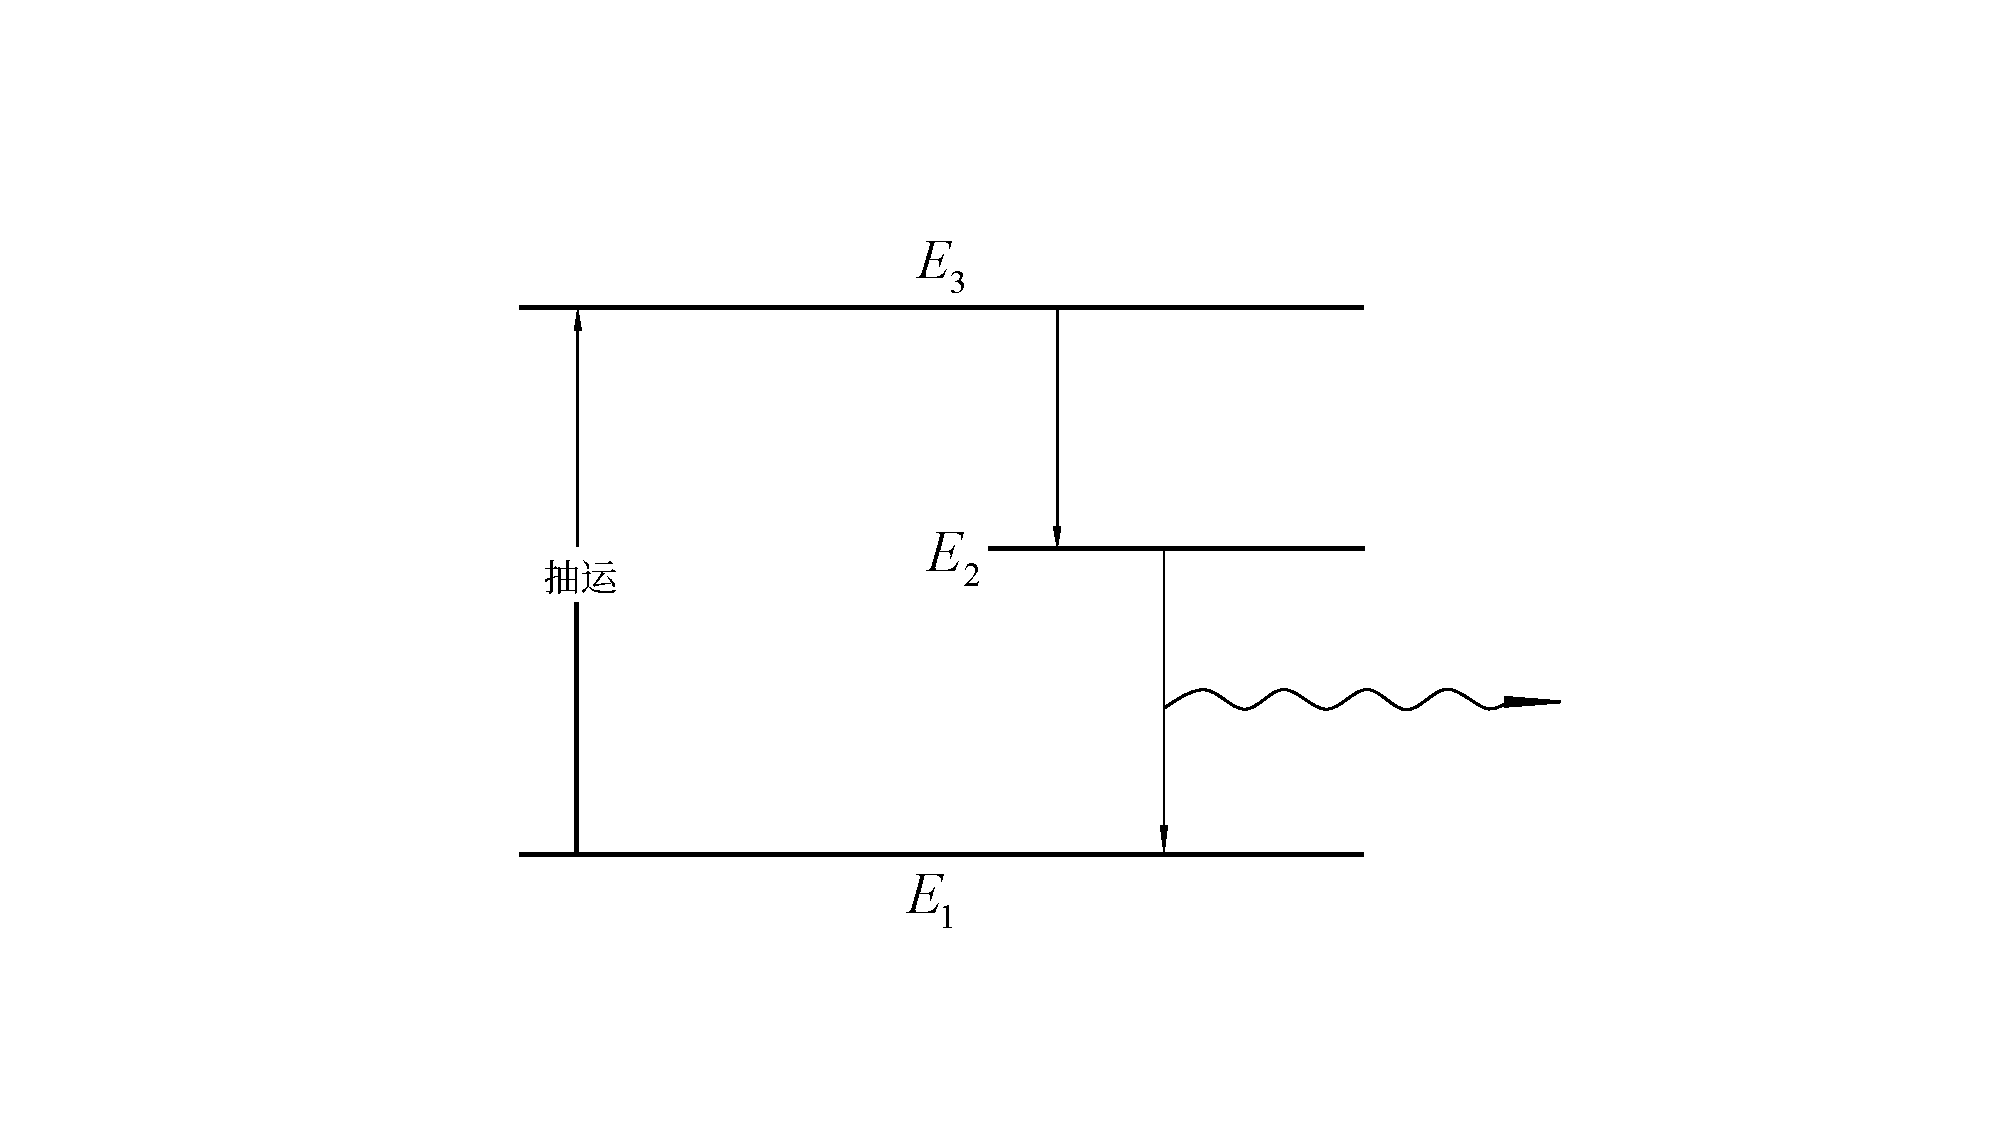
\includegraphics[width=4cm,clip]{QM file/figure/9-3}
	\caption{}\label{fig.9-3}
\end{wrapfigure}
第一代激光器是固体脉冲式,典型代表就是最早出现的红宝石激光器.红宝石是$\ce{Al_{2}O_{3}}$,渗有约0.04\%的\ce{Cr}.利用$\ce{Cr^{+++}}$离子的三能级系统产生激光.这三个能级如图\ref{fig.9-3}所示.用闪光氙灯照射红宝石棒,使$\ce{Cr^{+++}}$从基态能级$E_{1}$上升到$E_{3}$,这个过程称为抽运.$E_{3}$能级经由自发跃迁降到$E_{2}$(寿命约$10^{-7}\si{s}$),$E_{2}$是亚稳态,它与$E_{1}$间的自发跃迁寿命约$10^{-3}\si{s}$.$E_{2}$和$E_{1}$就是用来产生激光的工作能级.如来自氙灯的激发光足够强,在一次闪光时间内$(<10^{-3}\si{s})$就能在上能级$E_{2}$集聚起足够多的$\ce{Cr^{+++}}$离子,实现能级$E_{2}$,$E_{1}$间粒子数反转.红宝石棒的两端面做成平行反射面,(一端有10\%透射率,以获得激光输出)棒本身就是谐振腔.使$E_{2},E_{1}$间产生受激跃迁的最初光讯号就是自发跃迁产生的少数沿棒的轴向传播的光子$(\hbar\omega_{21})$,在两反射面间来回振荡,同时激发更多的$\ce{Cr^{+++}}$离子实现$E_{2}\rightarrow E_{1}$受激辐射,使腔内光讯号迅速放大,成为很强的平行光束,从一端射出这种激光器能量转换(氙灯光能$\rightarrow$激光输出)效率较低,在0.1\%以下.氙灯的每一次闪光,产生一次脉冲式激光(波长\num{694.3}\si{nm})输出,因为是脉冲式,输出激光的单色性并不很好.

能够连续地产生激光,单色性较好的是氦-氖激光器,它利用\ce{Ne}原子的特殊能级构造产生激光,能级图如图\ref{fig.9-4}所示.
\begin{figure}[!h]
	\centering
	\small
	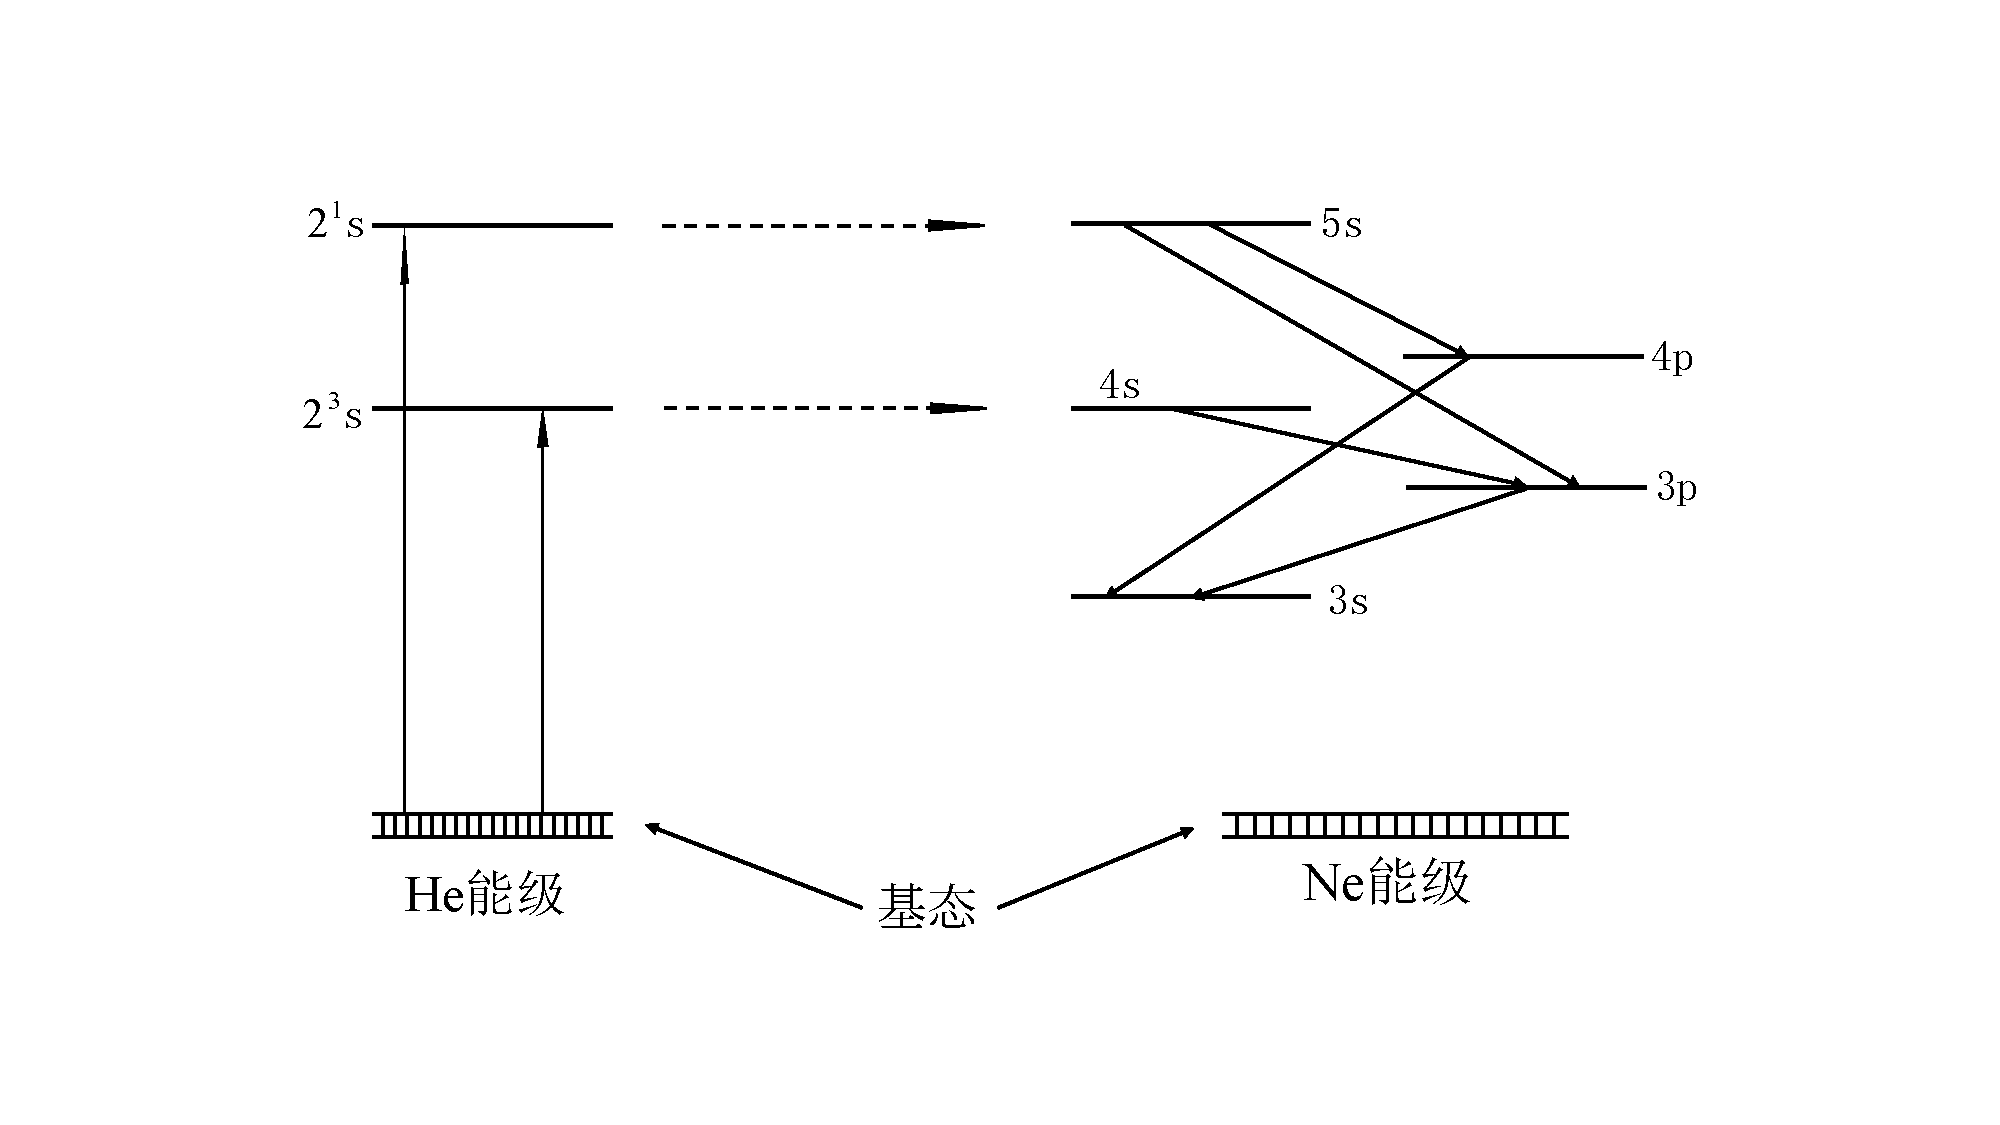
\includegraphics[width=6cm,clip]{QM file/figure/9-4}
	\caption{}\label{fig.9-4}
\end{figure}
\noindent 氦氖激光管中氦与氖约为5:1到10:1,管的两端加上$2\sim3\si{kV}$电压,使产生气体放电,电子的撞击使\ce{He}的一个电子被激发到$2^{1}\si{s}$或$2^{3}\si{s}$能级,再通过气体原子间的碰撞将能量转移给\ce{Ne}原子,使其处于单电子激发能级5s和4s(这两个能级恰好与\ce{He}的$2^{1}\si{s}$及$2^{3}\si{s}$能级接近,容易发生能量转移.)\ce{Ne}原子产生激光的能级跃迁是5s$\rightarrow$4p,5s$\rightarrow$3p,及4s$\rightarrow$3p,由于4p及3p能级原来是空的(\ce{Ne}原子集中在基态能级上),这样就很顺利地实现了上能级与下能级之间的原子数反转.完成受激辐射过程而到达4p及3p能级的原子,可以经由自发跃迁迅速降到3s能级,再经过碰撞降到基态,这样在下能级(4p,3p)就不会积累原子,所以产生激光的过程可以连续进行.造成谐振腔的反射镜可以放在管外,便于调节.氦氖激光有极好的单色性,如\ce{Ne}的5s$\rightarrow$3p跃迁产生的波长\num{632.8}\si{nm}的红光,$\frac{\Delta\nu}{\nu}\sim\num{1.6}\times10^{-11}$.最好的激光$\frac{\Delta\nu}{\nu}$仅$10^{-14}$.

激光器种类很多,发展很快,这里就不多介绍了.


% 能量-时间不确定度关系
\starthis\section[能量-时间不确定度关系]{能量-时间不确定度关系} \label{sec:09.06} % 
% \makebox[5em][s]{} % 短题目拉间距

微观过程的某些性质常可用“能量-时间不确定度关系”来解释.这个“不确定度关系”的一般表达方式是
\eqshort
\begin{empheq}{equation}\label{eq96.1}
	\Delta E\Delta t\gtrsim\hbar
\end{empheq}\eqnormal
$\Delta E,\Delta t$分别代表能量和时间的不确定度.由于能量是力学量,$\Delta E$可以尽量按精确的意义理解,其严格定义是
\begin{empheq}{equation}\label{eq96.2}
	(\Delta E)^{2}=\overline{E^{2}}-\overline{E}^{2}
\end{empheq}\eqshort
而时间并非力学量,对于过程的时间不确定度,一般仅作量级估算.因此\eqref{eq96.1}式也仅在量级意义上使用.我们将先讨论几个典型实例,借以说明\eqref{eq96.1}式的正确性,然后再稍作理论探讨.


\exa 原子自发辐射,初态$\varPsi_{2}\rightarrow$终态$\varPsi_{1}(E_{2}-E_{1}>0)$设在$t=0$制备好大量处于初态$\varPsi_{2}$的原子,然后就测量辐射的光子能量$E=\hbar\omega$.设跃迁$\varPsi_{2}\rightarrow\varPsi_{1}$的平均寿命为$\tau$,有效测量大致在$t=\tau$前完成,可取$\Delta t\sim\tau$.被测量的光子,其空间分布范围大致是$\Delta x\lesssim c\tau$,因此有动量不定值$\Delta p\sim\frac{\hbar}{\Delta x}\gtrsim\frac{\hbar}{c\tau}$,和能量不定值$\Delta E=c\Delta p\gtrsim\frac{\hbar}{\tau}$.结论是:测到的光子能量$\hbar\omega$并不严格地等于原子跃迁前后的能级差$(E_{2}-E_{1})$,而有不确定度$\Delta E$,而$\Delta E$,$\Delta t$满足\eqref{eq96.1}式.

表面看来,以上结论与能量守恒定律有矛盾,其实不然.到测得光子时为止,原子在终态$\varPsi_{1}$中停留的时间是有限的$(t\lesssim\tau)$所以终态并非严格意义下的定态,其能量值并不严格等于$E_{1}$,而有分布宽$\Delta E\gtrsim\frac{\hbar}{\tau}$,初态也有类似的能级宽度.初、终态的能级宽度正是光子能量不确定度的来由.总之,如某状态只在有限时间内存在,它就不是严格的定态,而有能量分布$\Delta E$.

\exa 在粒子物理研究中发现,能够自行蜕变的不稳定粒子,其质量都有不确定度$\Delta m$,它与蜕变的平均寿命$\tau$有关系
\begin{empheq}{equation}\label{eq96.3}
	\Delta m\cdot\tau\sim\frac{\hbar}{c^{2}}
\end{empheq}\eqnormal
用能量-时间不确定关系\eqref{eq96.1}式容易解释这个关系,因为粒子质量与相对论性质的能量有关系$E=mc^{2}$,所以$\Delta E=c^{2}\Delta m$,而寿命$\tau$正是时间不确定度$(\Delta t\sim\tau)$.

\exa 在单频微扰作用下原子从初态$\varPsi_{k}$(能级$E_{k}$)向终态$\varPsi_{f}$(能级$E_{f}$)跃迁.跃迁概率由\eqref{eq92.5}式表示.考虑终态能量连续的情形,对于$F_{fk}$相同而能量互相不同的终态,跃迁概率与初终态能级差$(E_{f}-E_{k})=\hbar\omega_{fk}$有关系
\begin{empheq}{align*}
	|C_{f}(t)|^{2} &\propto\frac{[1-\cos(\omega_{fk}-\omega_{o})t]}{(\omega_{fk}-\omega_{o})^{2}}	\\
	&\propto \frac{\sin^{2}[(\omega_{fk}-\omega_{o})t/2]}{(\omega_{fk}-\omega_{o})^{2}}
\end{empheq}\eqshort
$|C_{f}(t)|^{2}-\omega_{fk}$关系如图\ref{fig.9-5}所示.$\omega_{fk}$的有效分布宽度大致可以确定为$\Delta\omega_{fk}\sim\frac{2\pi}{t}$,因此终态能量不确定度约为$\Delta E_{f}\sim\frac{2\pi\hbar}{t}$,即
\begin{empheq}{equation}\label{eq96.4}
	\Delta E_{f}\cdot\sim2\pi\hbar
\end{empheq}\eqnormal

\begin{figure}[!h]
	\centering
	\small
	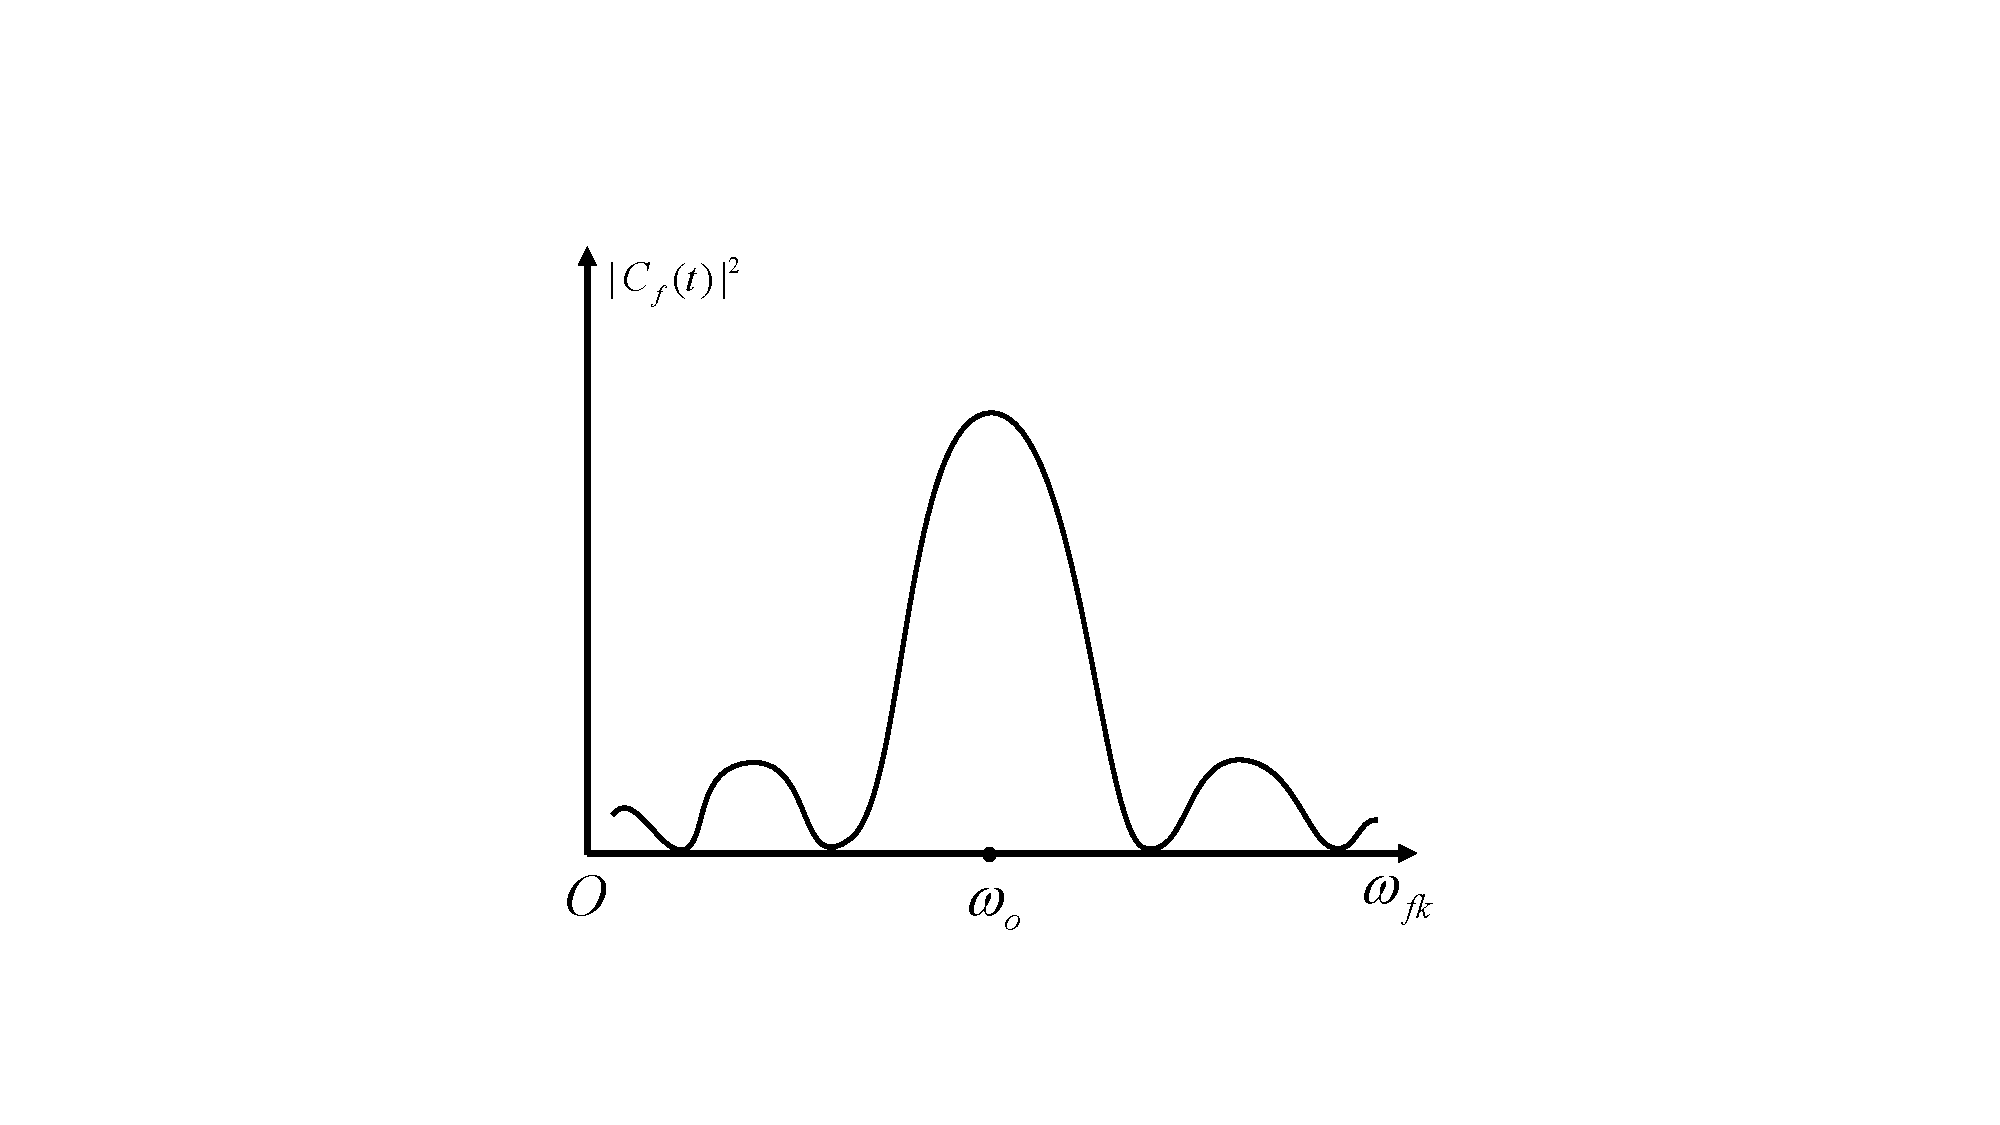
\includegraphics[width=5cm,clip]{QM file/figure/9-5}
	\caption{}\label{fig.9-5}
\end{figure}
\noindent 这里$t$相当于终态存在时间的不确定度,即$\Delta t$.造成终态能量不完全确定的原因是:微扰$H^{\prime}$既然只在有限时间内起作用,它实质上不是严格的单频微扰,其频谱宽度$\Delta\omega\gtrsim\frac{2\pi}{t}$,因此原子从$H^{\prime}$吸收的能量量子并不严格等于$\hbar\omega$,而有不确定度$\hbar\Delta\omega\gtrsim\frac{2\pi\hbar}{t}$,所以终态能量也有同样的不确定度.

在例1和例3中,$\Delta E$都很小,常可略去不计.例如例3,取$t\sim10^{-10}\si{s}$,则$\Delta E_{f}\sim\frac{\hbar}{t}\sim4\times10^{-5}\si{eV}$.$\S$\ref{sec:09.02}正是在忽略$\Delta E_{f}$的条件下,对跃迁速率作了近似处理,从而得出$E_{f}=E_{k}+\hbar\omega$的结论.但是例2中$\tau$有时非常小,$\Delta m$可以达到$m$的量级.

能量-时间不确定度关系的正确性是肯定的,对它的论证却并不统一.常见的一种论证是,取能量算符为$\hat{E}=i\hbar\frac{\partial}{\partial t}$,于是就有
\begin{empheq}{equation}\label{eq96.5}
	[t,\hat{E}]=[t,i\hbar\frac{\partial}{\partial t}]=-i\hbar
\end{empheq}\eqshort
再仿照$x-p_{x}$不确定关系的推导,得到
\begin{empheq}{equation*}
	\Delta E\cdot\Delta t\geqslant\frac{\hbar}{2}
\end{empheq}\eqnormal
这种论证显然不妥.我们姑且不去争论$t$是否可以作为算符对待,至少可以指出将$i\hbar\frac{\partial}{\partial t}$作为能量算符用于对易式的计算是不妥的,容易引申出种种谬论.例如,对于任何不显含$t$的算符$\hat{F}(\boldsymbol{r},\boldsymbol{p}$,显然有$\left[\hat{F},\frac{\partial}{\partial t}\right]=\frac{\partial\hat{F}}{\partial t}$,因此$F$是守恒量,等等.

利用狭义相对论中四维协变矢量的概念来论证能量-时间不确定关系也许是较好的办法.在相对论中,
\begin{empheq}{equation*}
	x_{\mu}=(x,y,z,ict),\quad p_{\mu}=\left(p_{x},p_{y},p_{z},\frac{iE}{c}\right)
\end{empheq}\eqshort
众所周知,利用$\hat{p_{x}}=-i\hbar\frac{\partial}{\partial x}$可以证明$x-p_{x}$不确定度关系:
\begin{empheq}{equation}\label{eq96.6}
	\Delta x\cdot\Delta p_{x}\geqslant\frac{\hbar}{2}
\end{empheq}
由于$\hat{p_{x}}=-i\hbar\frac{\partial}{\partial x}$也适用于相对论情形,所以\eqref{eq96.6}式也适用于相对论情形.$y-p_{y},z-p_{z}$间也有类似的不确定度关系.据此类推,$x_{4}=ict$与$p_{4}=\frac{iE}{c}$之间也应有不确定度关系:
\begin{empheq}{equation*}
	\Delta x_{4}\cdot\Delta p_{4}\geqslant\frac{\hbar}{2}
\end{empheq}
亦即
\begin{empheq}{equation} \label{eq96.7}
	\Delta t\cdot\Delta E\geqslant\frac{\hbar}{2}
\end{empheq}\eqnormal
在量级的意义上,\eqref{eq96.7}式与\eqref{eq96.1}式并无不同



% 习题
\begin{exercises}
	
\exercise 设$t<0$时体系处于基态$\varPsi_{1}$,$t>0$时受到逐渐增强再逐渐消退的外来微扰$H^{\prime}(x,t)$作用,
\begin{empheq}{equation*}
	H^{\prime}(x,t)=\frac{F(x)}{[\tau^{2}+(t-t_{0})^{2}]},\quad \frac{t_{0}}{\tau}\gg1
\end{empheq}

设$t_{0}$很大,满足$\dfrac{(E_{2}-E_{1})t_{0}}{\hbar}\gg2\pi$.求微扰消退后$(t\rightarrow\infty)$体系处于各激发态$[\varPsi_{n}(x)]$的概率.
	
\exercise 某体系(能量算符$H_{0}$)只有两个能级(非简并的),$E_{2}-E_{1}=\hbar\omega>0$,设$t<0$时处于基态$\varPsi_{1}$.$t>0$时受到外来作用,能量算符变成$H=H_{0}+H^{\prime}$,设$H^{\prime}$不含$t$,矩阵元为
\begin{empheq}{align*}
	\langle\varPsi_{1}|H^{\prime}|\varPsi_{1}\rangle&=\langle\varPsi_{2}|H^{\prime}|\varPsi_{2}\rangle=0,	\\
	\langle\varPsi_{1}|H^{\prime}|\varPsi_{2}\rangle&=\langle\varPsi_{2}|H^{\prime}|\varPsi_{1}\rangle=\hbar\nu
\end{empheq}

试严格求解薛定谔方程,求$\varPsi(t)$.如在任意$t>0$时刻测量$H_{0}$之值,测得$H_{0}=E_{2}$的概率等于什么?

[提示:先求出$H$的本征函数$\varPsi_{\alpha},\varPsi_{\beta}$,本征值$E_{\alpha},E_{\beta}$,再将$\varPsi(t)$表示成也$\varPsi_{\alpha},\varPsi_{\beta}$的叠加,求出$\varPsi(t)$后,再表示成$\varPsi_{1},\varPsi_{2}$的叠加.]

\exercise 上题中,设$H^{\prime}$是微扰,即设$\nu\ll\omega$,求$t>0$时刻测得$H_{0}=E_{2}$的概率,与微扰论结果[\eqref{eq91.12}式]比较.

\exercise $t=0$时电子的自旋取值为$S_{z}=\dfrac{\hbar}{2}$,$t>0$时受到沿正$x$轴方向的磁场$(\boldsymbol{B})$作用,作用势为
\begin{empheq}{equation*}
	H^{\prime}=\frac{e B}{m_{e}c}S_{z}=\hbar\omega\sigma_{x},\quad \omega=\frac{e B}{2m_{e}c}
\end{empheq}

视$H^{\prime}$为微扰,用\eqref{eq91.12}式计算$t>0$时测得$S_{z}=-\dfrac{\hbar}{2}$的概率.微扰论计算公式成立的条件是什么?(本题是在简并态之间的跃迁问题,请与7-20题结果对照.)

\exercise 电荷为$e$(或$-e$)质量为$m$的一维谐振子,(a) 写出电偶极跃迁选择定则.(b) 求自发跃迁速率公式(初态$\varPsi_{n}$).
	
\exercise 电荷为$e$(或$-e$)质量为$m$的三维各向同性谐振子,[用直角坐标系,以$\varPsi_{n1}(x)\varPsi_{n2}(x)\varPsi_{n3}(x)$作为能量本征函数.](a) 求电偶极跃迁选择定则,(b) 求自发跃迁速率公式.(设初态量子数$n_{1}=n_{2}=n_{3}=n$,考虑向一切可能的终态跃迁速率之和.)(c) 取$n_{1}=n_{2}=n_{3}=1$,如谐振子是电子,$\hbar\omega=1\si{eV}$,求初态平均寿命.如谐振子是质子,$\hbar\omega=1\si{MeV}$,求初态平均寿命.
	
\exercise 处于无限深平底势阱中的带电粒子,求其电偶极跃迁选择定则.
	
\exercise 考虑自旋轨道耦合,原子中价电子(最外层电子)定态波函数取$(H,\boldsymbol{L}^{2},\boldsymbol{J}^{2},J_{z})$共同本征函数,量子数$(nljm_{j})$.对于价电子的自发跃迁(电偶极跃迁),证明选择定则是
\begin{empheq}{equation*}
	\Delta l=\pm1,\quad \Delta j=0,\pm1,\quad \Delta m_{j}=0,\pm1
\end{empheq}

[提示:利用公式$\boldsymbol{\sigma}(\boldsymbol{\sigma}\cdot\boldsymbol{r})+(\boldsymbol{\sigma}\cdot\boldsymbol{r})\boldsymbol{\sigma}=2r$,以及7-15题证明的公式.注意$\boldsymbol{r},\boldsymbol{\sigma}\cdot\boldsymbol{r}$及$Y_{lm}$的宇称性.要着重证明$\Delta j=\pm2$的跃迁是禁止的.]

\exercise 大量氢原子均处于基态,而且电子自旋均沿正$z$轴方向极化,即电子处于$(n,l,m,m_{s})=\left(1,0,0,\dfrac{1}{2}\right)$状态,亦即$(n,l,j,m_{j})=\left(1,0,\dfrac{1}{2},\dfrac{1}{2}\right)$状态.今用电场沿$\pm z$轴方向偏振的线偏振光照射这些原子,造成1s$\rightarrow$2p能级跃迁,忽略2p$_{1/2}$态与2p$_{3/2}$态的能量差.[取相同的径向波函数$R_{21}(r)$]试利用上题证明的选择定则确定终态$(n=2)$量子数$ljm_{j}$的可能取值,并计算终态为2p$_{1/2}$和2p$_{3/2}$的分支比(原子数之比).
	
\exercise 以磁场$\boldsymbol{B}(t)$作用于原子,引起价电子状态的跃迁,求量子数$(lmm_{s})$及$(ljm_{j})$的选择定则.
	
\end{exercises}
